\documentclass{article}

%\usepackage{natbib}

% Tables
\usepackage{siunitx}	% Simple units and decimal point alignment in tables
\usepackage{booktabs}	% Pretty booktabs
\usepackage{multirow}	% Multi- rows and columns + cell-specific positioning
\usepackage{rotating}	% Rotated tables
\usepackage{longtable}	% Multi-page spanning tables
\usepackage[table,xcdraw]{xcolor}   % Color and colored tables
\usepackage{lscape}     % Tables in landscape mode

% Packages
\usepackage[utf8]{inputenc}	% Tillåter å ä ö som direkt input
\usepackage{graphicx}	% Figures
\usepackage{subcaption}	% Subfigures
\usepackage{amsmath}	% Alignment of equations
\usepackage{lipsum} 	% Lorem Ipsum
\usepackage{setspace}	% Switch between simple- and double spacing
\usepackage{framed}		% Environment that frames everything in it
\usepackage{hyperref}	% Hyperlinks, websites, e-mail
\usepackage{enumitem}	% Spika bullet symbols för \itemize och stil för \enumerate
\usepackage{pdfpages}   % Include pdf pages
\usepackage[T1]{fontenc}	% Tillåter tolkning av å ä ö m.m.
\usepackage[a4paper,textwidth=500pt,textheight=700pt]{geometry}	% Spikar marginaler
\usepackage{float}	% Allows more advanced positioning of floats
\usepackage[parfill]{parskip}	% Uses spacing instead of indents on line breaks
\usepackage{minted}
\usepackage{textgreek}      % Grekiska tecken utan math mode

%\usepackage[colorlinks=true, allcolors=blue]{hyperref}
%\usepackage{pgfplotstable}	% Import excel tables from .csv files
%\usepackage{lmodern}
%\usepackage{csquotes}
%\usepackage{fancyhdr}
%\usepackage[style=numeric,sorting=none, maxbibnames=9, maxcitenames=2, backend=biber]{biblatex}
%\usepackage[dvipsnames]{xcolor}
%\usepackage{gensymb}

%\usepackage{amssymb}
%\usepackage{parskip}
%\usepackage{titlesec}
%\usepackage{multicol}
%\usepackage{blindtext}
%\usepackage{titlesec}
%\usepackage{caption}
%\captionsetup{font=small, labelfont=bf, tableposition=top}

\begin{document}

\includepdf[pages={1}]{pages/cover.pdf}
%\newpage
%\thispagestyle{empty}
%\mbox{}

\newpage
\setcounter{page}{1}
\thispagestyle{empty}
\section*{Abstract}
The clinical severity of Covid-19 varies greatly between individuals, and all underlying risk factors are not yet well understood. Previous studies have shown Covid patients to be enriched with autoantibodies against type I interferons, suggesting autoimmunity may be an underlying factor of susceptibility to severe disease. In this project, the interplay between severe Covid-19 and autoimmunity was investigated in 114 Swedish patients, sampled in April-May 2020 as well as longitudinal re-samplings 4 and 8 months later, using the infrastructure of the Human Protein Atlas and the SciLife lab autoimmunity and serology profiling unit. First, 16 patients with few comorbidities were analyzed for autoantibodies at a near proteome-wide scale using planar microarrays, after which a custom antigen panel was assembled based on observed reactivities and literature studies. The antigen panel was implemented in a 384-plex suspension bead array which was run for all patient samples and a control group. Among the Covid patients, 23 antigens were called as differentially reactive and 8 of them were proposed as relevant to immunoregulation or Covid pathogenesis. The results partially replicated previous findings of autoimmunity directed to type I interferons and offer a list of candidate autoantigens for further inquiries.

\vspace{1cm}
\section*{Sammanfattning}
Allvarlighetsgraden av sjukdomen Covid-19 varierar kraftigt mellan individer och alla underliggande riskfaktorer är ännu inte förstådda. Tidigare studier har påvisat Covidpatienter som överrepresenterade med autoantikroppar mot typ I interferoner, vilket förespråkar autoimmunitet som en möjlig underliggande riskfaktor till att utveckla allvarlig Covid. I detta projekt användes infrastrukturen av det mänskliga proteinatlasprojektet och enheten för autoimmunitets- och serologiprofilering på SciLife lab för att undersöka samspelet mellan allvarlig Covid-19 och autoimmunitet i 114 st svenska patienter inlagda under april-maj 2020, samt från uppföljningsprover 4 resp. 8 månader senare. Till en början undersöktes 16 patienter med låg grad av samsjukdom för förekomst av autoantikroppar mot proteomet i stort med hjälp av mikroarrayer. En panel av antigen sammanställdes därefter baserat på resultaten och litteraturstudier. Panelen implementerades som en 384-plex kulsuspensionsarray vilken kördes för alla patientprover samt en kontrollgrupp. Ibland Covidpatienterna klassades 23 st antigen som överrepresenterade, varav 8 st avsågs relevanta för immunoreglering eller sjukdomsförlopp. Resultaten visades delvis återskapa tidigare fynd av autoimmunitet riktad mot typ I interferoner och erbjuda en lista av potentiella autoantigen för vidare efterforskningar.

\vspace{2cm}
\subsubsection*{Keywords}
Covid-19, SARS-CoV-2, Autoimmunity, Autoantibodies, Cytokines, Interferons

\newpage
\tableofcontents

\newpage
\section{Introduction}
\subsection{Covid-19 and autoimmunity}
Covid-19, is an infectious disease caused by the coronavirus SARS-CoV-2 which since the end of 2019 has spread into a pandemic with over 166,860,000 reported cases and 3,460,000 deaths \cite{who_report}, of which over 1,058,000 cases and 14,300 deaths are in Sweden \cite{fohm}.

Despite the relatively low case fatality rate, the severity and clinical outcome of the disease varies greatly between individuals. Even though several important risk factors such as age, sex and various underlying health conditions have been identified, many people still appear to be disproportionately affected (or unaffected) by the disease – implying all underlying risk factors are not yet well understood \cite{susceptibility}. Furthermore, it has been established that the most severe damage caused by Covid- 19 is done by a dysregulated immune response, rather than the virus itself \cite{dysregulated}.

A proposed contributor to this clinical variability is autoimmunity which can be hypothesised as an underlying factor of susceptibility to severe disease as well as a tendency to develop serious complications post infection, so called "Long Covid". In autoimmunity, the immune system recognizes a native substance as foreign; such "autoreactive" substances are referred to as "autoantigens" and may lead to the production of specifically targeted "autoantibodies" (aABs) as well as a large variety of health complications and disease states. Most people exhibit autoreactivity to at least some native substances \cite{aa_healthy}, but in some cases these reactivities may cause or predispose illness.

In Covid patients specifically, there have been demonstrations of autoimmunity directed towards cytokines – the molecules responsible for cross-talk and communication within the immune system. Interferons are a type of cytokine which specifically prevent and combat viral infections \cite{ifn}. Bastard \textit{et al} have shown that patients with severe Covid-19 are significantly enriched with autoantibodies against type I interferons and present evidence that these autoantibodies drive the severity of the disease \cite{bastard}. Similarly, Zhang \texit{et al} have shown that patients with non-functioning type I interferon responses, due to inborn errors, are more severely afflicted \cite{zhang_inborn_2020}. Both articles indicate that the genetic or autoimmune phenocopies of deficient or non-functional type I interferons are a driver of morbidity and mortality in Covid-19.

\subsection{The Human Protein Atlas}
The Human Protein Atlas (HPA) \cite{hpa} is an extensive, Swedish-based program aiming to map the localization of all human proteins on a cell, tissue and organ level by integrating various omics technologies. This endeavour uses polyclonal antibodies, targeting different human protein epitopes, at a near proteome-wide scale. The HPA antibodies are produced by immunizing rabbits with synthetic peptides called protein epitope signature tags (PrESTs). 

The PrESTs are expressed in \textit{Escherichia coli} and are designed based on the following bioinformatical criteria \cite{prest}:

\begin{itemize}
    \item Represent a predicted human protein, based on ensembl \cite{ensembl}
    \item Less than 60\% sequence homology to other human proteins over a 50 aa sliding window
    \item Less than 8 aa sequence homology to other human proteins over a 10 aa sliding window
    \item No predicted transmembrane regions of signal peptides
    \item Between 25-150 amino acids long (average 80 aa)
\end{itemize}

Since 2003, the production of HPA antibodies has yielded over 42,000 PrESTs representing over 19,000 human proteins. Because the PrESTs are designed to represent a human protein epitope they can, besides the application of antibody production via immunization, also be coupled to planar or bead arrays to be utilized in autoimmunity assays.

\subsection{Autoimmunity profiling technologies}
In an autoimmunity assay, a panel of putative autoantigens is put in contact with a sample which is surveyed for the presence of autoantibodies directed towards their respective autoantigen in the panel. Once the autoantibodies are bound the total reactivity of each antigen can be evaluated, commonly by use of a secondary, anti-human detection antibody coupled to a fluorophore which is then measured optically.

\subsubsection{Planar microarray}
Autoimmunity assays can be performed on planar microarrays by coupling different antigens to ordered spots on a microarray slide. The broadest planar microarray within the HPA infrastructure, colloquially referred to as the "42k-array", contains the entire HPA PrEST collection and consists of two glass slides containing 21,000 PrESTs each \cite{42k}. While the antigens included in this array is a comprehensive representation of the complete set of the gene-derived proteome, there is no inherent possibility of sample multiplexing, so the throughput is limited to one sample or one sample pool per assay.

\subsubsection{Suspension Bead Array}
In a suspension bead array (SBA), antigens are instead coupled to magnetic beads in solution. Unlike the planar microarray where the identities of the antigens are retained by a spatial position in the array, the identity of each bead is spectrally discerned through a combination of different wavelengths and corresponding intensities of internal bead dyes \cite{xmap}. Because all different beads can be pooled, allowing for antigen multiplexing, it is possible to scale the assay to run on hundreds or thousands of samples. The Luminex MagPlex beads and FlexMap 3D instrument allows for multiplexing of 384 antigens prepared in a four-plate protocol.

\subsection{The Community study}
The Community (short for Covid Immunity) study \cite{community, fas2} follows a cohort of over one hundred Covid patients and over two thousand healthcare workers from Danderyd university hospital. The purpose of the study is primarily to evaluate the longitudinal prevalence of anti-SARS-CoV-2 antibodies in the healthcare workers in connection with exposure and symptoms.

The 118 patients were sampled at multiple instances during hospital admission in April-May 2020 and invited for longitudinal re-sampling in September 2020 and January 2021. The initial sampling and two follow-up samplings are referred to as phases 1, 2 and 3 respectively.

At the time this project was initiated, the ethical framework only allowed for broad, prognostic biomarker discovery within the patients in the Community cohort, while the personnel were limited to investigations of SARS-CoV-2 antigens, specifically. Because this project aims at investigating the interplay between Covid and autoimmunity, only the patient samples were used.

\subsection{Project outline}
The intent of this project is to explore the autoimmunity profiles of the Covid patients of the Community study and compare them to a control group, leveraging the available technologies and infrastructure of the SciLife lab autoimmunity profiling facility and the Human Protein Atlas.

First, a subset of representative patients from phase 1 will be selected and analyzed via the broad, planar microarray. Secondly, based on the reactive PrESTs of the microarray and genes described in literature as relevant to the interplay between autoimmunity and Covid pathogenesis, an antigen panel will be constructed and implemented as a custom, 384-plex suspension bead array. Lastly, this SBA, which is more targeted than the planar microarray but highly scalable, will be utilized for all patients of all phases of the study as well as a control group.

The goal of the project is to generate a list of candidate autoantigen which are differentially reactive in Covid patients compared to the control group. These findings will also be put in relation to those of Bastard \textit{et al}, by investigating in particular the observed autoreactivity towards type I interferons. The data from phases 2-3 will enable longitudinal analysis in a subset of patients, which can be used to investigate how reactivity towards antigens may change over time.

\section{Materials and methods}
\subsection{Planar microarray}\label{method_42}
The limited throughput of the planar microarray protocol was sought to be increased in order to include more subjects and hence capture more autoreactivities. Previous endeavours have shown that the samples of up to four patients can be pooled for the analysis while still yielding interpretable results. For this reason, it was decided to run the analysis on four pools containing four samples each.

Because the exploratory analysis of the autoreactivities of these 16 patients was expected to broadly affect the composition of the custom antigen panel, it was deemed important to minimize the number of comorbidities.  We reasoned that it would be more interesting to investigate the patients that had become inexplicably ill, rather than the ones whose disease severity could be attributed to any of a vast assortment of comorbidities.

\subsubsection{Sample selection}
In consultation with a collaborating clinician, the clinical data of 115 hospitalized Covid patients was manually surveyed. Variables of interest were age, sex, previously known health conditions (comorbidities) and disease severity. The care unit submission type was deemed an appropriate categorical marker of disease severity: submission to intensive care (IVA) meant the patients had at some point required invasive assisted respiration, while submission to intermediary care (IMA) meant the patients had at some point required non-invasive assisted respiration.

The presence and variation of comorbidities was very high in the cohort, and isolating patients with no previously known comorbidities and IVA/IMA submission yielded only 12 patients which could be stratified by sex and clinical severity into three pools. The first pool consisted of four men submitted to IVA, the second of four men submitted to IMA and the third of four women submitted to IVA or IMA. In this third pool, one woman had to be excluded and was replaced with a woman with documented asthma. In contrast, the fourth and final pool was filled with “wildcard” patients, selected manually by the collaborating clinician. Of these, two had multiple sclerosis (MS) and were undergoing treatment with the drug Mabthera, one had Guillain-Barre syndrome (GBS) contracted in connection to Covid and one was immunosuppressed.

\begin{table}[H]
\caption{Four pools containing four patient samples each were selected based on known comorbidities, sex and disease severity.}
\label{42k_pools}
\begin{center}
{\renewcommand{\arraystretch}{1.2}
\begin{tabular}{|c|cc|c|c|}
\hline
\textbf{Pool} & \multicolumn{2}{c|}{\textbf{Comorbidities}} & \textbf{Sex} & \textbf{Severity} \\ \hline\hline
1 & \multicolumn{2}{c|}{\cellcolor[HTML]{A9D08E}} &  & IVA (critical) \\ \cline{1-1} \cline{5-5} 
2 & \multicolumn{2}{c|}{\multirow{-1}{*}{\cellcolor[HTML]{A9D08E}11 w. none}} & \multirow{-2}{*}{Male} & IMA (severe) \\ \cline{1-1} \cline{3-5} 
3 & \multicolumn{1}{p{140pt}}{\cellcolor[HTML]{A9D08E}} & \cellcolor[HTML]{FFD966}1 w. asthma & Female & \cellcolor[HTML]{D9D9D9} \\ \cline{1-4}
4 & \multicolumn{2}{c|}{\cellcolor[HTML]{F4B084}Autoimmune disease or immunosuppression} & \cellcolor[HTML]{D9D9D9}Mixed & \multirow{-2}{*}{\cellcolor[HTML]{D9D9D9}Mixed} \\ \hline
\end{tabular}
}
\end{center}
\end{table}

\subsubsection{Experimental procedure}
The samples, consisting of heat-treated plasma were moved from -80$^{\circ}$C storage, thawed overnight in -20$^{\circ}$C storage and thawed prior to handling in 4$^{\circ}$C. From each sample, 15 µL was transferred to its respective pool for a total volume of 60 µL per pool.

An assay buffer was prepared, consisting of 10 ml phosphate buffer solution (09-9400-100, Medicago) + 0.1\% Tween20 (BP337-500, Fisher) (PBST), 0.3 g 3\% Bovine Serum Albumin (B2000-500, Saveen Werner) (BSA) and 0.5 g 5\% milk (70166-500G, Sigma).

Because each planar microarray consists of 2 glass slides containing ~21,000 PrESTs each, the eight required glass slides (in-house batch 5) were retrieved from 8$^{\circ}$C storage, mounted to a slide rack and dipped in milliQ several times. They were then dried in a slide centrifuge and transferred to horizontal slide mounts for handling. Microarray coverslips (100 \textmu l, LifterSlip)  were cleaned with ethanol, distilled water and blow dried.

Each sample pool was diluted 1:25 (to obtain 1:100 dilution for each sample) with 160 \textmu g His$_6$ABP/ml in assay buffer. The diluted pools were then incubated for 15 min in an Elmi Intelli-Mixer RM-2L, program UU at 30 rpm. To each slide, 85 µL of its respective pool was applied in a vertical line after which the chamber cover was placed on top to allow the liquid to distribute uniformly across the entire slide. All slides were then incubated in RT for 1 h.

The slides were then put into 50 ml Falcon tubes filled with 0.1\% PBST to loosen the chamber covers which were removed using a pincer. The slides were the transferred to a slide rack which was washed by submerging in 0.1\% PBST for 5 min on a shake table at 80 rpm.

The slides were then incubated with ~1:40 000 Hen anti-His6ABP IgY (25 mg/ml, Immunotech HPA), submerged in PBST on a shake table at 80 rpm for 1 h, after which they were washed twice.

The slides were then incubated with ~1:15 000 goat anti chicken Alexa 555 (2 mg/ml, A-21437, Invitrogen) and goat anti-human IgG (H+L) Alexa 647 (2 mg/ml, A21445, Life Technology), submerged in PBST on a shake table at 80 rpm for 1 h. Finally, they were washed twice with PBST, once with PBS, dipped in MilliQ and dried in a slide centrifuge.

\subsubsection{Image analysis}
The slides were scanned using an InnoScan 1100AL (Innopsys) with the parameters width: 22,000, length: 72,000, red channel: PMT 950; Power 100 and Green channel: PMT 750; power 75. The green channel (532 nm) corresponds to the detection of the His$_6$ABP tag, i.e. PrESTs, while the red channel (635 nm) corresponds to the detection of human IgG.

The scanned images were then interpreted using the software GenePix 5.1 (Molecular Devices) and a grid detailing the spatial coordinates of each feature was manually fitted to the image. The settings were the default 2-colour mode settings for the mode "find irregular features" with the parameters composite pixel intensity: 300 MFI, resize features during alignment: feature diameter min 33\% - max 150\%.

For each slide, the result of the automated feature alignment tool was briefly manually inspected and any discoveries of calls which were deemed erroneous were flagged as such. The highest ranked intensities (approximately a dozen per slide) were also systematically inspected and curated the same way.

Once inspected and manually curated, each feature alignment was converted to a data structure in .gpr-format detailing the identity and metrics of each spot therein.

\subsection{Antigen panel assembly}\label{method_panel}
\subsubsection{Control beads}\label{method_control_beads}
The 384-plex SBA would include four control beads, leaving room for 380 antigens in the customized panel. The control beads were:

\begin{itemize}
    \item An "empty" bead with no coupled antigen, included as a negative control for the array.
    \item A bead coupled with anti-human IgG Fc antibodies, included as a positive control for all samples containing human IgG.
    \item A bead coupled to Epstein–Barr virus nuclear antigen 1 (EBNA1) which is expected to exhibit a variable reactivity across human samples.
    \item A bead coupled to the His$_6$ABP tag present on all PrESTs, included as a negative control to demonstrate that the samples have been depleted of anti-His$_6$ABP antibodies and that any activity exhibited by a PrEST is not due to the tag, but the PrEST itself.
\end{itemize}

\subsubsection{Full length type I interferons}
Two full length type I interferons (IFN\textalpha 2A and IFN\textomega 1) were purchased and included in the panel (SRP4594-100UG, SRP3061-100UG, Sigma).

This was done partially in order to replicate the findings of Bastard \textit{et al} \cite{bastard} but also to cross-reference the reactivities of the full length interferons to those of the PrESTs. If reactivity is seen for the former but not the latter, it would indicate the PrESTs do not fully represent the same, reactive epitopes as the full length proteins. Reactivity among the full length proteins and differential reactivity among the PrESTs might also indicate which epitopes are targeted, specifically.

\subsubsection{PrEST antigen}
The remaining 378 antigen in the panel would consist of PrESTs.

A literature study was conducted and a list was compiled containing genes relevant to the interplay between autoimmunity and Covid or other infectious diseases. These 24 genes were 13 subtypes of interferon \textalpha{}, interferons \textomega, \textbeta, \textkappa, \textepsilon{} \cite{bastard}, \textgamma{} \cite{lit_ifng}, interleukins 6 \cite{lit_il6}, 17A, 17F , 22 \cite{lit_il17_22}, 23 and Granulocyte-macrophage colony-stimulating factor (CSF2) \cite{lit_il23_csf2}.

A list of all genes which had been represented by reactive PrESTs in the planar microarray analysis as well as all genes from the literature study was compiled and input to LIMS to yield a list of corresponding PrESTs IDs (HPRR) and antigen IDs (HPRA). HPRR identifies the PrEST as a bioinformatical construct while HPRA identifies the batch of the PrEST as a physically expressed antigen. Rows with missing HPRA were removed and the remaining rows were deduplicated with respect to HPRR. This list was, in turn, run on an in-house script to generate a data frame containing the physical locations of the antigens which was then supplemented with information from the microarray results.

The goal was to include all PrESTs which had been reactive in the planar microarray analysis as well as all PrESTs representing genes from the literature list. Because all PrESTs were not expected to be available, a "backup" list of PrESTs was constructed for filling up whichever space remained in the panel. These were PrESTs that represented proteins with an immunological function and extracellular localization, and that had been represented in the planar microarrary analysis by some other reactive PrEST, sorted by descending reactivity.

The code for generating the location list can be found in appendix \ref{panel_localize}.

\subsubsection{Final composition}
Available PrESTs were collected from in-house storage as well as the facilities of Atlas Antibodies in Bromma. The collection and final antigen panel is summarized in table \ref{method_panel_comp}.

\begin{table}[H]
\centering
\caption{Composition of the final antigen panel in terms of antigen type, motivation for inclusion and storage type. Physically, the panel consisted of 328 tubes and 52 plate wells from 37 different plates.}
\label{method_panel_comp}
{\renewcommand{\arraystretch}{1.3}
\begin{tabular}{|rl|rp{8.2cm}|rl|}
\hline
\textbf{\#} & \multicolumn{1}{l}{\textbf{Type}} & \textbf{\#} & \multicolumn{1}{l}{\textbf{Comment}} & \textbf{\#} & \textbf{Storage} \\ \hline\hline
\multirow{6}{*}{378} & \multirow{6}{*}{PrEST} & \multirow{2}{*}{325} & \multirow{2}{*}{Reactive \textgreater{}4 SD in microarray analysis} & 281 & Tube \\ 
 &  &  &  & 44 & Plate \\ \cline{3-6} 
 &  & \multirow{2}{*}{25} & \multirow{2}{*}{Represents proteins mentioned in   literature} & 21 & Tube \\ 
 &  &  &  & 4 & Plate \\ \cline{3-6} 
 &  & \multirow{2}{*}{28} & \multirow{2}{*}{\parbox{8.2cm}{Represents proteins that have other reactive PrESTs, immunological function and extracellular localization}} & 24 & Tube \\  
 &  &  &  & 4 & Plate \\ \hline\hline
2 & Full length protein & 2 & IFN\textalpha 2A and IFN\textomega & 2 & Tube \\ \hline\hline
4 & Control beads & 4 & Empty, anti-human IgG Fc, EBNA1, His$_6$ABP & 4 & Tube \\ \hline\hline
\textbf{384} & \multicolumn{1}{l}{} & \textbf{384} & \multicolumn{1}{l}{} & \textbf{384} & \\ \hline
\end{tabular}
}
\end{table}

\subsection{Suspension Bead Array}
The experimental procedure was carried out based on the in-house standard operating procedure (SOP) for SBA autoimmunity profiling (version 2.2), variations of which have been used for similar projects \cite{aa_healthy, aa_csf}.

\subsubsection[Antigen dilution]{Antigen dilution\\{\normalfont\slshape\normalsize The 380 antigens and four controls are diluted and transferred to four 96-well plates.}}\label{method_antigen_dilution}

The finished antigen panel was formatted and fed into an in-house script (v11) which generated three work list files (.gwl) compatible with the liquid handling system used (Tecan Freedom EVO) as well as an updated antigen position list and worktable layouts. The updated list detailed the expected source and destiny positions of all tubes and wells and the volumes required to achieve their target concentrations. Some wells would be diluted manually.

First, 4x50 ml MES buffer (M2933-100G, Sigma) was thawed overnight at 4$^{\circ}$C. The antigens and control reagents were also thawed at 4$^{\circ}$C before handling. The control reagents consisted of rabbit anti-human IgG (309-005-082, Jackson), EBNA1 (ab138345, abcam), His6ABP (Human Protein Atlas, batch conc. 5.78 mg/ml).

The liquid handling system was inspected, loaded with tips and pumped with system liquid (dH$_2$O) twice to remove air bubbles. The worktable was loaded with four 10 ml tubes of MES buffer and the appropriate amount was distributed to each well of the four 96-well plates.

For the antigen dilution carried out by the liquid handling system, 322 antigen tubes were transferred to 48-tube holders in the order specified by the updated list, vortexed, spun down (2000 RPM, 1 min) and loaded onto the worktable. Two different worktable layouts were used to include all tubes in up to four tube holders at a time. Similarly, 34 antigen plates containing 49 antigens of interest were vortexed, spun down (stacked two at a time, 1000 RPM, 1 min) and loaded in three different layouts running on 12, 12 and 10 plates at a time.

Three antigen plate wells (IDs 375-377) and three tubes (IDs 14, 70, 71) had to be transferred manually due to low well volume and incompatible tube format. An additional antigen was manually transferred to it's tube because it had not been included in the original script run (ID 380). The two full length proteins were hydrolyzed with 100 \textmu l milliQ according to manufacturers' instructions, vortexed and transferred manually to destiny plates along with the three control reagents. The fourth control well was simply filled with buffer, totaling at 384 wells.

For all antigens, the full-length proteins and His6ABP, the final concentrations were 0.4 mg/ml. For the rabbit anti-human IgG and EBNA1 the final concentrations were 1.8 and 1.35 mg/ml, respectively. The destiny plates were sealed, vortexed, spun down (2000 RPM, 1 min) and transferred to overnight storage in 4$^{\circ}$C.

\subsubsection[Bead coupling]{Bead coupling\\{\normalfont\slshape\normalsize The beads are chemically activated and the antigens are coupled to the beads.}}

Four 96-well plates containing 40 \textmu l Luminex MagPlex bead stock solution (500 000 beads) per well were prepared and stored in 4$^{\circ}$C wrapped in foil. The MES buffer was used, as well as 3x50 ml AB buffer (S3139-250G, Sigma) thawed in 4$^{\circ}$C overnight and 5 ml 10xBRE (11 112 589 001, Roche) thawed in 4$^{\circ}$C the same day.

Four aliquots of 65 mg EDC (Proteochem) as well as stock NHS (24510, Thermo Scientific) were transferred from -20$^{\circ}$C to RT for 30 min. Aliquots of NHS were made and weighed at 66.7, 66.7, 66.1 and 69.9 mg before being put on silica beads along with the EDC aliquots for 30 min.

The diluted antigen plates were vortexed and spun down (2000 RPM, 1 min) and the bead plates were moved to RT and spun down (2000 RPM, 1 min).

\textit{Due to the nature of the reagents used, the following steps are time sensitive and were performed twice, for two plates at a time.}
\begin{quote}
First, the plates were washed by adding 80 \textmu l AB buffer via automated multipipette and draining on magnet using a BioTek EL406 washer dispenser. A further 50 \textmu l AB buffer was then added via automated multipipette.

For each plate, one aliquot of EDC and NHS were diluted separately in AB buffer to 50 mg/ml after which 1200 \textmu l of both solutions were combined with a further 3600 \textmu l AB buffer. The resulting 6000 \textmu l activation solution was transferred to a trough and dispensed at 50 \textmu l (or 0.5 mg EDC/NHS) per well into the corresponding bead plate using an automated multipipette.

The plates were then sealed, vortexed and incubated at RT in a hooded plate shaker (650 RPM, 20 min).

After incubation, the plates were pulsed at 1000 RPM and washed twice on magnet in 2x100 \textmu l MES buffer using an automated multipipette for dispensation and BioTek for aspiration.

The diluted antigens (100 \textmu l per well) were then added to the bead plates. The plates were then sealed, vortexed and incubated at RT in a hooded plate shaker (650 RPM, 2x1h with vortexing between).
\end{quote}

Storage buffer was prepared by adding 45 ml milliQ and 50 \textmu l ProClin (48912-U, Sigma) to the thawed 5 ml 10xBRE buffer. 

\textit{The following steps were also performed twice, two plates at a time due to the time lag introduced earlier.}
\begin{quote}
After incubation, the plates were washed twice in 100 \textmu l 0.05 PBS-T on magnet using BioTek. Using an automated multipipette, 50 \textmu l storage buffer was added to each well off-magnet. The plates were then sealed and vortexed.
\end{quote}
Following protocol completion for all four plates, they were vortexed, pulsed at 1000 RPM and stored at 4$^{\circ}$C until bead pooling 6 days later.

The complete list of bead couplings can be found in appendix \ref{sba_full}.

\subsubsection[Bead pooling]{Bead pooling\\{\normalfont\slshape\normalsize The beads are pooled into one 96-plex tube per plate.}}\label{bead_pooling}

The plates were moved from storage and pulsed at 1000 RPM. The beads were then re-suspended in the plate wells by repeated pipetting using a manual multi-channel pipette.

\textit{For each plate:}
\begin{quote}
    A flat-bottomed, slide washer tray was placed, at a tilt, on a plate magnet after which the whole bead plate volume was transferred to the side of the tray in contact with the magnet. The pipette tips were reused for the whole transfer to limit bead loss. The wells were washed with an additional 50 \textmu l storage buffer each and were then transferred to the tray in the same manner.
    
    The tray was re-positioned horizontally on the magnet and 7 ml storage buffer was carefully aspirated from the opposite side of the beads and transferred to a 15 ml tube on magnet. The beads were re-suspended in remaining ~3 ml storage buffer in the tray by repeated aspiration and transferred to a 5 mL LoBind tube on magnet where the beads were allowed to settle.
    
    The entire tray was washed thrice using 700 \textmu l supernatant from the 5 ml LoBind tube. The volume of the tube was then visually adjusted to 1.25 ml, resulting in a 96-plex SBA pool.
\end{quote}

From each 96-plex pool, 300 \textmu l was transferred after vortexing to a 1.5 ml LoBind tube, corresponding to a 1200 \textmu l 384-plex SBA pool.

\subsubsection[Pre-run assay tests]{Pre-run assay tests\\{\normalfont\slshape\normalsize The coupling of the beads is evaluated.}}

In order to evaluate the quality of the SBA, a control assay run was performed on 21 wells which included three different types of tests:
\begin{itemize}
    \item A coupling test, in which a hen anti-His$_6$ABP antibody is added in PBST to bind the His$_6$ABP tag present on all PrESTs (n=378) and the His$_6$ABP control bead. The purpose of the test is to verify that the antigens have successfully coupled to the beads. The test is performed in triplicate and with one PBST control.
    \item A sample test, in which commercial plasma is added in assay buffer. The reactivity profile may vary depending on the plasma, but reactivity is expected for the anti-human IgG control bead and likely for the EBNA1 control bead as well. The purpose of the test is to verify that running on plasma yields acceptable results. The test is performed in triplicate and with one assay buffer control.
    \item A number of specific antigen tests, in which HPA antibodies directed towards specific PrESTs are added in PBST to verify that they bind their specific targets on the beads. In this project, six HPA antibodies are used. Three of them target IFN\textalpha2A, IFN{\textomega} and both respectively. They were included to evaluate binding to the full length interferons present in plate 4 as well as the IFN{\textalpha2A/\textomega} PrESTs in pool 1. The remaining three target arbitrarily chosen PrESTs in pool 2, 3 and 4. Each specific antigen test is performed in duplicate and with one PBST control. A summary of the chosen antibodies and their targets can be seen in table \ref{specific_table}.
\end{itemize}

\begin{table}[H]
\centering
\caption{Summary of the antibodies used for the specific test. All antibodies targeting beads in plate 1 were chosen for also evaluating reactivity to the full length interferons in plate 4, while the antibodies targeting plates 2-4 were chosen arbitrarily.}
\label{specific_table}
\begin{tabular}{@{}lllll@{}}
\toprule
\textbf{HPA antibody} & \textbf{Target PrEST} & \textbf{Target bead} & \textbf{Target genes} & \textbf{Target plate} \\ \midrule
HPA045659 & HPRR3360041 & 32 & IFNA various, IFNW1 & 1 \\
HPA047557 & HPRR3360040 & 33 & IFNA various & 1 \\
HPA053957 & HPRR3780122 & 89 & IFNW1 & 1 \\
HPA031823 & HPRR2800004 & 147 & SNAP29 & 2 \\
HPA058595 & HPRR3720498 & 288 & ELF4 & 3 \\
HPA059220 & HPRR3560056 & 294 & FJX1 & 4 \\ \bottomrule
\end{tabular}
\end{table}

The test solutions were prepared: For the coupling test, 0.5 \textmu l hen anti-His$_6$ABP (produced in-house) was added to 5 ml PBST for a 1:10 000 dilution. For the sample test, 300 \textmu l assay buffer w/o His$_6$ABP, consisting of phosphate buffer solution (09-9400-100, Medicago) + 0.1\% Tween20 (BP337-500, Fisher) (PBST), 3\% Bovine Serum Albumin (B2000-500, Saveen Werner AB) (BSA) and 5\% milk (70166-500G, Sigma) was combined with 8.54 \textmu l 5.78 mg/ml His$_6$ABP solution (in-house) to yield assay buffer including 160 \textmu g/ml His$_6$ABP. Of this assay buffer, 250 \textmu l was combined with 1 \textmu l commercial plasma (K2EDTA mixGender, cat\#HUMANPLK2PNN, lot\#HMN192452, BioIVT) for a 1:250 dilution. For each specific antigen test, 0.5 \textmu l of the corresponding HPA antibody was added to 250 \textmu l PBST for a 1:500 dilution.

To each of the 21 wells, 5 \textmu l vortexed 384-plex SBA solution was added. To each of the 18 testing wells, 45 \textmu l of the respective test solutions were added and to the 3 control wells, the same solutions without primary antibodies were added. The plate was sealed, vortexed and incubated on shake (650 RPM, 1h). The plate was then pulsed at 1000 RPM and washed thrice in 100 \textmu l PBST using BioTek.

The detection antibodies were diluted: For the coupling test, 0.5 \textmu l 0.5 mg/ml R-PE conjugated donkey F(ab')2 fragment anti-hen IgY (703 116 155, Jackson) was diluted in 500 \textmu l PBST. For the sample test, 1 \textmu l 0.5 mg/ml R-PE conjugated goat F(ab')2 fragment anti-human IgG (eBioScience) was diluted in 625 \textmu l PBST. For the specific antigen test, 1 \textmu l 1 mg/ml R-PE-conjugated anti rabbit IgG (111-116-144, Jackson) was diluted in 2000 \textmu l PBST.

To each well, 50 \textmu l of the corresponding detection antibody solution was added. The plate was then sealed, vortexed and incubated on shake (650 RPM, 30 min). The plate was then pulsed at 1000 RPM, washed thrice in 100 \textmu l PBST and finally dispensed with 100 \textmu l PBST using BioTek.

The plate was lastly transferred to a Luminex Flexmap 3D instrument. It was run using a 96-well protocol with a 60 second timeout per well.

\subsubsection{Sample selection}\label{sba_sample_selection}
The Covid-19 patient cohort consisted of samples from phases 1-3 of the Community study \cite{fas2} i.e. 118 patient samples from April-May 2020, 60 follow-up samples from September 2020 and 51 additional follow-up samples from January 2021. In phase 1 many patients had been sampled multiple times and for these cases the last sample in the series was used. Three replicates consisting of commercial plasma and one empty control well were to be included in each of the four 96-well assay plates.

The 229 Covid-19 patient samples and 16 plate controls left space for 139 control samples. The control samples originated from a large in-house study called EIMS, consisting of multiple sclerosis (MS) patients and healthy controls (cohort ID MSC\_6). To make the sample transfer as simple as possible it was decided that the 139 controls would be transferred plate-wise from approximately one and a half of the twenty-four 96-well plates in storage.

It was thus of interest to find the control plates which would be most appropriate to use. The cohort sample information was downloaded from the laboratory information system (LIMS) and processed in R \cite{R} using package tidyverse \cite{tidyverse}. The code can be found in appendix \ref{code_control_wrangle}. No single plate had more than 35\% men or 21\% healthy men so it was deemed relevant to find the one and a half plates which would maximize these parameters to strive for an even gender ratio and a large healthy control group. It was decided to use plate 14 and the second half of plate 16, together corresponding to 34\% men and 60\% healthy controls. The composition of all samples used in the assay can be seen in table \ref{sba_samples}.

\begin{table}[H]
\centering
\caption{Samples used for the SBA run. For the Covid patients, statistics of sex and age were obtained from published data \cite{fas2}.}
\label{sba_samples}
{\renewcommand{\arraystretch}{1.3}
\begin{tabular}{|rlrl|cc|}
\hline
\multicolumn{1}{|l}{\textbf{\#}} & \textbf{Type} & \textbf{\#} & \textbf{Group} & \textbf{\% men} & \textbf{mean age} \\ \hline\hline
\multirow{3}{*}{229} & \multicolumn{1}{l|}{\multirow{3}{*}{Case}} & 118 & Hospital admission & \multicolumn{1}{c}{\multirow{3}{*}{69}} & \multirow{3}{*}{56} \\ \cline{3-4}
 & \multicolumn{1}{l|}{} & 60 & 4 month follow-up & \multicolumn{1}{c}{} &  \\ \cline{3-4}
 & \multicolumn{1}{l|}{} & 51 & 8 month follow-up & \multicolumn{1}{c}{} &  \\ \hline\hline
\multirow{3}{*}{139} & \multicolumn{1}{l|}{\multirow{3}{*}{Control}} & 84 & Healthy & \multicolumn{1}{c}{\multirow{3}{*}{34}} & \multirow{3}{*}{40} \\ \cline{3-4}
 & \multicolumn{1}{l|}{} & 54 & MS & \multicolumn{1}{c}{} &  \\ \cline{3-4}
 & \multicolumn{1}{l|}{} & 1 & Unknown & \multicolumn{1}{c}{} &  \\ \hline\hline
\multirow{2}{*}{16} & \multicolumn{1}{l|}{\multirow{2}{*}{Plate control}} & 12 & Commercial plasma & \multicolumn{1}{c}{\multirow{2}{*}{-}} & \multirow{2}{*}{-} \\ \cline{3-4}
 & \multicolumn{1}{l|}{} & 4 & Empty & \multicolumn{1}{c}{} &  \\ \hline\hline
\multicolumn{1}{|l}{\textbf{384}} &  & \textbf{384} &  & \multicolumn{1}{c}{\textbf{56}} & \textbf{50} \\ \hline
\end{tabular}
}
\end{table}

A graphical layout was constructed for performing plate-wide transfers from the six crude sample plates to the four assay plates using a semi-automatic pipettor and control wells were arbitrarily but evenly distributed across the plates (see appendix \ref{sample_layout}). 

\subsubsection{Sample dilution}
First, two sets of assay buffer were prepared: one with His$_6$ABP (set 1) and one without (set 2). Set 1 consisted of 50 ml phosphate buffer solution (09-9400-100, Medicago) + 0.1\% Tween20 (BP337-500, Fisher) (PBST), 1.5 g 3\% Bovine Serum Albumin (B2000-500, Saveen Werner) (BSA) and 2.5 g 5\% milk (70166-500G, Sigma). Set 2 was prepared by adding 1.19 ml 4.4 mg/ml His$_6$ABP (in-house) to 15 ml of set 1 solution. Set 1 and set 2 were transferred (49 \textmu l and 60 \textmu l per well) to two sets of four skirted 96-well PCR-plates using an automated multipipette.

The two crude control sample plates were thawed from -80$^{\circ}$C to -20$^{\circ}$C overnight and then put on ice with the remaining four crude sample plates. Once thawed, they were vortexed and spun down (3000 RPM, 1 min).

In accordance with the layouts in appendix \ref{sample_layout}, 1 \textmu l of each of the selected samples was transferred from the six crude plates to the four set 1 plates. Plate-wide transfers were performed using a CyBio SELMA semi-automatic pipettor while some wells were transferred manually to allow a seamless merge of the source layouts as well as an even distribution of replicates and control wells within the destination plates.

The set 1 plates and crude plates were sealed, vortexed and centrifuged (3000 RPM, 1 min) and the crude plates were then returned to -20$^{\circ}$C storage overnight to be returned to -80$^{\circ}$C later. The CyBio SELMA semi-automatic pipettor was then used to directly transfer 15 \textmu l per well from the set 1 plates to the set 2 plates, which were then sealed, vortexed, centrifuged (3000 RPM, 1 min) and incubated on a shake table (80 RPM, 1h).

\subsubsection{Assay run}
Of the 384-plex SBA pool, $\sim$1095 \textmu l remained from the bead pooling (section \ref{bead_pooling}). An additional 280 \textmu l was added from each vortexed 96-plex pool to yield $\sim$2215 \textmu l 384-plex pool. An automatic stepper pipette was used to transfer 5 \textmu l per well of the 384-plex SBA pool to a 384-well Greiner assay plate, 16 wells at a time with vortexing between.

The set 2 plates were centrifuged (3000 RPM, 1 min) and transferred, one plate per quadrant, to the assay plate using a Tecan Freedom Evo liquid handling system. The assay plate was then sealed, vortexed and incubated in a hooded plate shaker (650 RPM, 2x1h with vortexing between).

To crosslink any bound autoantibodies to the beads, 28.5 ml PBST and 1.5 ml paraformaldehyde (43368, Alfa Caesar) (PFA) were mixed to a 0.2\% solution. Using a BioTek EL406 washer dispenser, the assay plate was washed thrice in PBST, after which 50 \textmu l of the 0.2\% PFA was added to each well. The assay plate was then sealed, vortexed and incubated in a hooded shake table (650 RPM, 10 min).

Detection antibody solution was prepared by diluting 40 \textmu l 0.5 mg/ml goat anti-human IgG Fc (12-4998-82, eBioscience) in 25 ml PBST for a final concentration of 0.8 \textmu l/ml. The assay plate was pulsed (1000 RPM) and again washed thrice in PBST using the BioTek, after which 50 \textmu l of the diluted detection antibody was added using an automated multipipette. The plate was then sealed, vortexed and incubated in a hooded plate shaker (650 RPM, 30 min). Finally, the plate was pulsed (1000 RPM), washed thrice in PBST and dispensed with 60 \textmu l PBST per well using the BioTek.

The plate was ran on a Luminex Flexmap 3D instrument with 45 second timeout and a double wash every 96$^{th}$ sample.

\section{Data analysis}
 The data analysis was carried out in R \cite{R} using the packages tidyverse \cite{tidyverse}, limma \cite{limma}, ggbeeswarm \cite{ggbeeswarm} and ggpubr \cite{ggpubr}. 
 
\subsection{Planar microarray}\label{data_planar}
The code is available in appendix \ref{code_42k}. Prior to this analysis, results were run on an in-house script to generate quality reports and metrics of e.g. database similarity, i.e. how frequently a certain reactivity had been observed in previous runs.

\subsubsection{Filtering}
The image analysis data for each slide was imported in .gpr-format and merged into a data frame. The database similarity was incorporated from the in-house script result. The data was filtered to remove spots which were either flagged in the image analysis, non-PrESTs, smaller than 30 pixels or whose PrEST detection signal was lower than 10 standard deviations above that of the spot background. For replicate spots (i.e. spots presenting the same PrEST), only the highest signal spot was kept.

\subsubsection{Normalization}
The signal was defined as the pixel median fluorescence intensity (MFI) of the spot subtracted with the MFI of its local background (see equation \ref{mfi}). The main, normalized, signal measure used in this report is referred to as standard deviations above baseline (SDs), defined as the difference between the spot MFI and the mean MFI of the slide, divided by the MFI standard deviation of the slide (see equation \ref{sds}). The statistics are used on a per-slide basis to compensate for differing plasma concentrations across the pools as well as technical variation between the slides.

\textit{for spot i on slide j:}
\begin{equation}\label{mfi}
    MFI_{i,j} = MFI^{foreground}_{i,j} - MFI^{background}_{i,j}
\end{equation}
\begin{equation}\label{sds}
    SDs_{i,j} = \frac{MFI_{i,j} - mean(MFI_j)}{SD(MFI_j)}
\end{equation}

\subsubsection{Annotation}
Gene name, gene descriptions and Uniprot ID for each PrEST was incorporated from an in-house database. Gene Annotation (GO) \cite{GO} information was then downloaded via Uniprot \cite{uniprot} and incorporated as well. After manual inspection of the GO-annotated results, two lists of keywords were constructed to flag PrESTs which represented proteins with an immunological function or which were extracellularly accessible, see appendix \ref{kw}.

\subsubsection{Reactivity calling}
A threshold of 4 SDs were applied to determine which PrESTs were reactive. The final results included 352 reactive spots corresponding to 332 unique PrESTs.

\subsection{Suspension Bead Array}
The code for the pre-run assay tests can be found in appendix \ref{code_tests} and the code for the analysis of the main run can be found in appendix \ref{code_sba}.

\subsubsection{Pre-run assay tests}
The Luminex bead count and MFI for each well and bead ID were merged with the test metadata for easier handling.

The bead count across all beads was surveyed. For the coupling test and sample test, the mean MFIs of the test triplicates were calculated for each bead ID and compared to the negative controls. For the specific antigen tests, the mean MFIs of the HPA antibody duplicate samples were calculated for each bead ID and the signal profiles were surveyed.

\subsubsection{Data structuring}
The Luminex data consisted of the measured bead count and median bead fluorescence intensity (MFI) for each sample and antigen. These two 384x384 matrices were pivoted into a long table containing 147,456 observations. All available patient information was downloaded from LIMS and merged into a comprehensive data structure. Similarly, the same methodology as section \ref{data_planar} was employed to collect information about all beads and their contents. The observations table was merged with both the sample information and the antigen information to yield a complete data structure containing all relevant information for each observation.

In order to assess to quality of the SBA, all observations of the control beads were inspected.

\subsubsection{Rationale of statistical methods}\label{statrat}
When making group comparisons of autoimmunity profiles, especially in a discovery-oriented endeavour, the majority of observations across samples and antigens are expected to be non-reactive. For this reason classical quantitative approaches, such as the Wilcoxon Rank Sum Test or t-test, tend to measure small but consistent group differences in the non-reactive bulk of observations rather than the relatively few, reactive outliers which actually represent the property of interest.

A more suitable approach is to set a threshold, separating observations to reactive and non-reactive respectively. For the observations of each antigen, separating by group and reactivity results in a contingency table were the statistical significance can be computed with Fisher's exact test, indicating whether the antigen is differentially reactive in a particular group.

Setting a threshold to determine which observations are reactive and not is far from obvious: samples may differ in plasma concentration and quality, resulting in different per-sample background levels. Likewise, the different antigens may be subject to vastly different background levels due to differences in concentration or binding availability.

In order to separate all differetially reactive observations from their respective backgrounds, one approach is to make the observations directly comparable by normalizing each observation by it's own background and then applying a single threshold across all observations. In order to quantitatively compare the observations of a specific antigen across multiple samples, we can normalize by sample background. Likewise, in order to compare the observations of a specific sample across multiple antigens we can normalize by the antigen background. This is based on the assumption that the majority of observations across samples and antigens are nonreactive. This assumption is expected to hold true for all observations except those which measure the positive control beads.

One metric which can represent the background level across a set of values is the MAD, defined as the median absolute deviation of the values from the median of the set.
\begin{center}
    \textit{For $\{d_1,d_2,d_3...\} \in D$}
\end{center}
\begin{equation}
    MAD(D) = median( \{ | d_i - median(D) | \} )
\end{equation}

We can normalize the observations per sample, per antigen or both - defining the signal as the number of MADs from the median.

\begin{center}
    \textit{For observation $MFI_{i,j}$ of sample $s_i \in S$ and antigen $ag_j \in Ag$}
\end{center}
\begin{equation}\label{mads_sample}
    MADs^{S}_{i,j} = \frac{MFI_{i,j} - median(s_i)}{MAD(s_i)}
\end{equation}
\begin{equation}\label{mads_ag}
    MADs^{Ag}_{i,j} = \frac{MFI_{i,j} - median(ag_j)}{MAD(ag_j)}
\end{equation}
\begin{equation}\label{2mads}
    MADs^{S,Ag}_{i,j} = \frac{MFI_{i,j} - median(s_i) - median(ag_j)}{MAD(s_i)*MAD(ag_j)}
\end{equation}


\subsubsection{Normal- and binarization}
First, all observations associated with a bead count < 30 were removed (n = 771). Then, the median and MAD was calculated with respect to each sample and antigen (excluding the positive control beads). The normalized signals for each observation were then calculated as described in equations \ref{mads_sample}-\ref{2mads}.

The threshold for reactivity was set to 1.5 $MADs^{S,Ag}$ based on the profile of the negative control beads. The subsequent number of reactivities per sample and antigen were surveyed.

\subsubsection{Group comparison}\label{method_group_comp}
Four patients were excluded from the Covid cohort (affecting four samples from phase 1 and one sample from phase 2) due to having tested negative for SARS-CoV-2 during hospital admission and one sample was excluded from the EIMS cohort due to missing data. The remaining samples of the EIMS cohort, consisting of MS patients and healthy controls, were treated as a single, non-Covid group for the sake of simplicity and statistical power.

For each phase of Covid patients and each antigen, the numbers of reactive and nonreactive samples were compared to those in the control group using Fisher's Exact Test, set to evaluate enriched reactivity in the Covid group.

The significance threshold was set to p < 0.05.

\section{Results}
\subsection{Planar microarray}\label{42k_results}
The four arrays represented a total of 235,008 observations, of which 117,730 (50.1\%) remained after filtering. The effects of the per-glass normalization are visualized in figure \ref{42k_corr}. The normalized distributions of significant signals across the glasses are shown in figure \ref{42k_boxplot}. The distributions were not found to significantly differ between the glasses.

Of the 235,008 filtered spots, 352 spots (0.30\%) representing 332 unique PrESTs showed a reactivity above 4 SDs. The full list of significantly reactive spots is available in appendix \ref{42k_results}.

\begin{figure}[H]
	\centering
    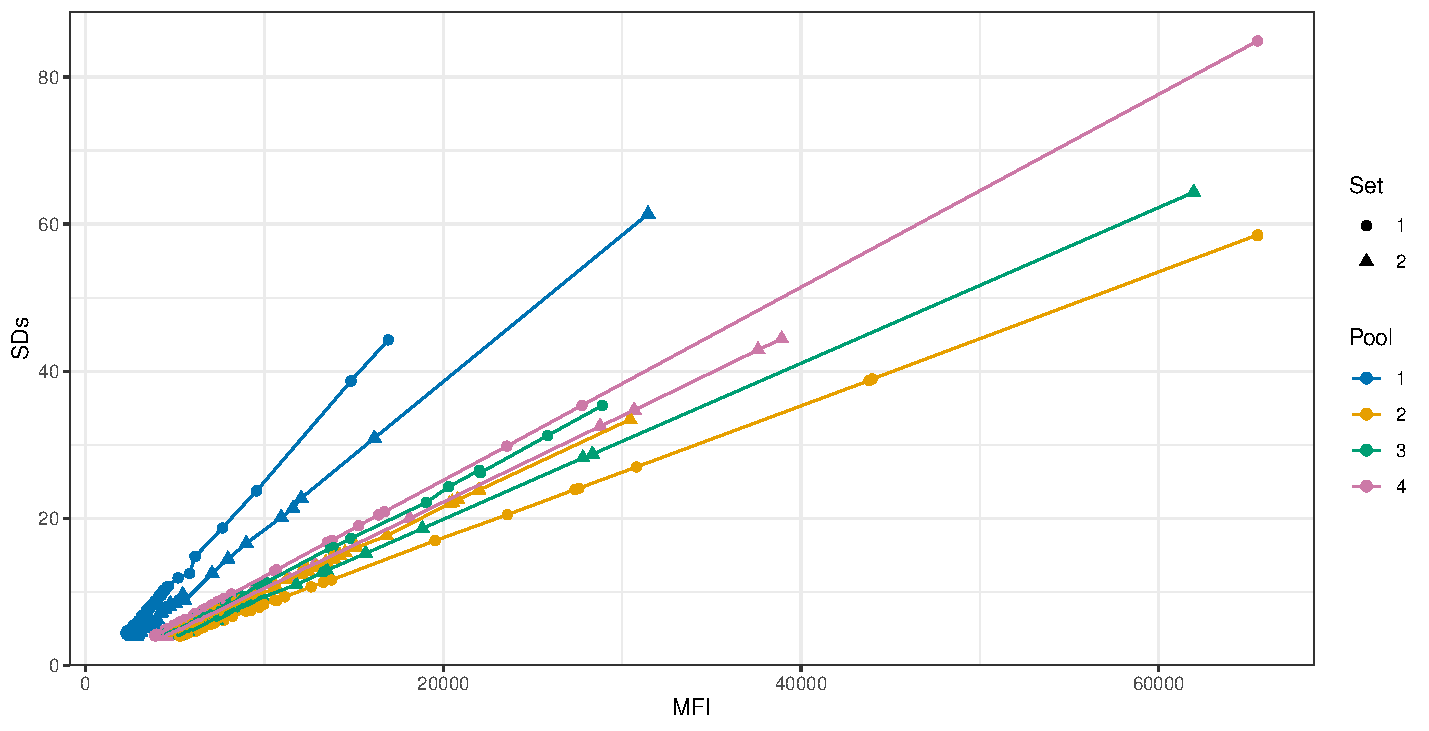
\includegraphics[width=0.9\linewidth]{figures/42k_corr.pdf}
    \caption{The x-axis shows the foreground pixel median signal intensity (MFI) of the reactive spots and the y-axis shows the corresponding normalized signal (SDs) as explained in equation \ref{sds}. The points are colored by pool, shaped by slide set and shown connected by both to highlight the different correlations.}
    \label{42k_corr}
\end{figure}
\begin{figure}[H]
	\centering
    \hspace*{3.5mm}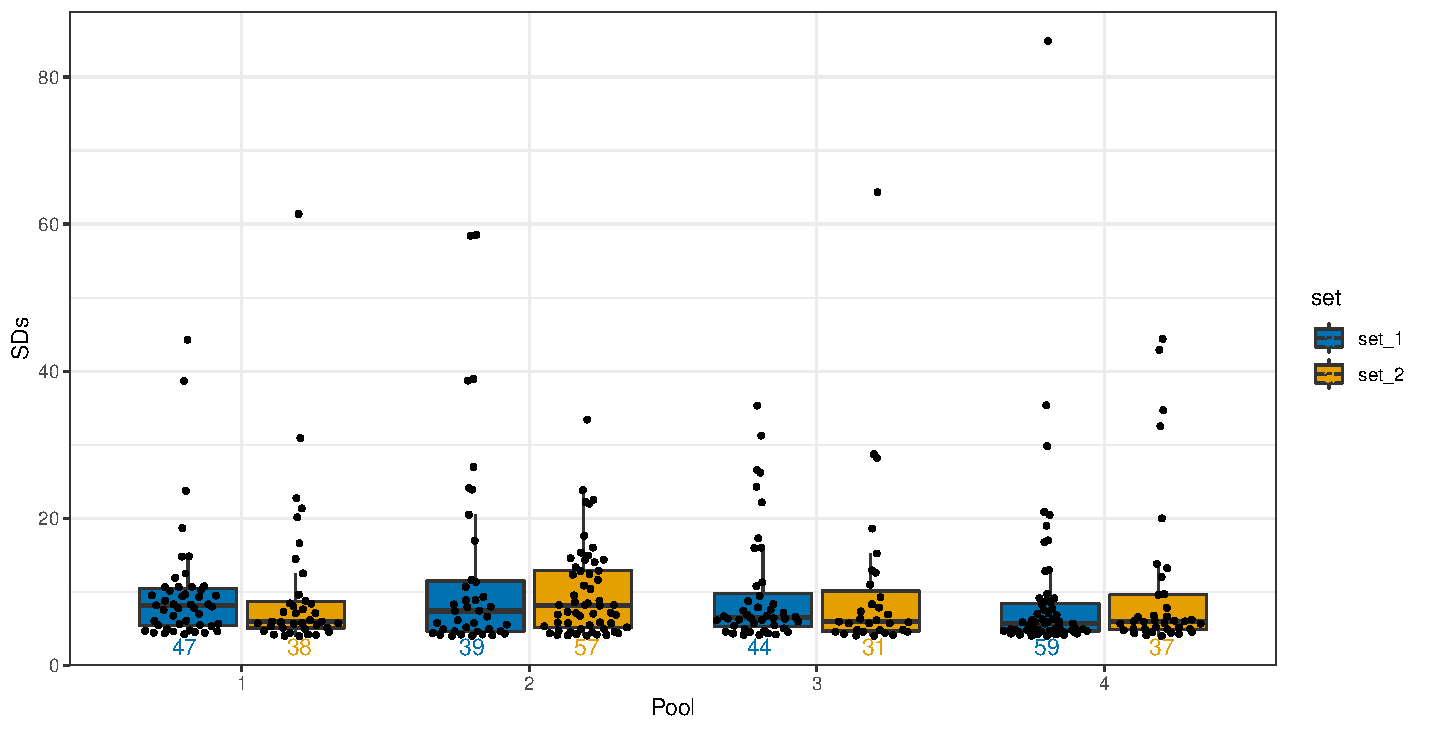
\includegraphics[width=0.9\linewidth]{figures/42k_boxplot.pdf}
    \caption{Boxplots and swarm plots showing the normalized signal of the significant observations for each pool and set. The number of observations is shown below each distribution.}
    \label{42k_boxplot}
\end{figure}

\subsection{Suspension Bead Array}
\subsubsection{Pre-run assay tests}
The bead count across all bead IDs can be seen in figure \ref{count_384}. Only five beads (IDs 51, 73, 88, 221, 257) had observations with counts below 30 and only one bead (ID 221) had a count median below 30, at 29. The median bead counts per plate were 134, 112, 124 and 114 for plates 1-4 respectively. The plate-wide differences were not estimated to necessitate any volume adjustment to the 384-plex pooling.

\begin{figure}[H]
	\centering
	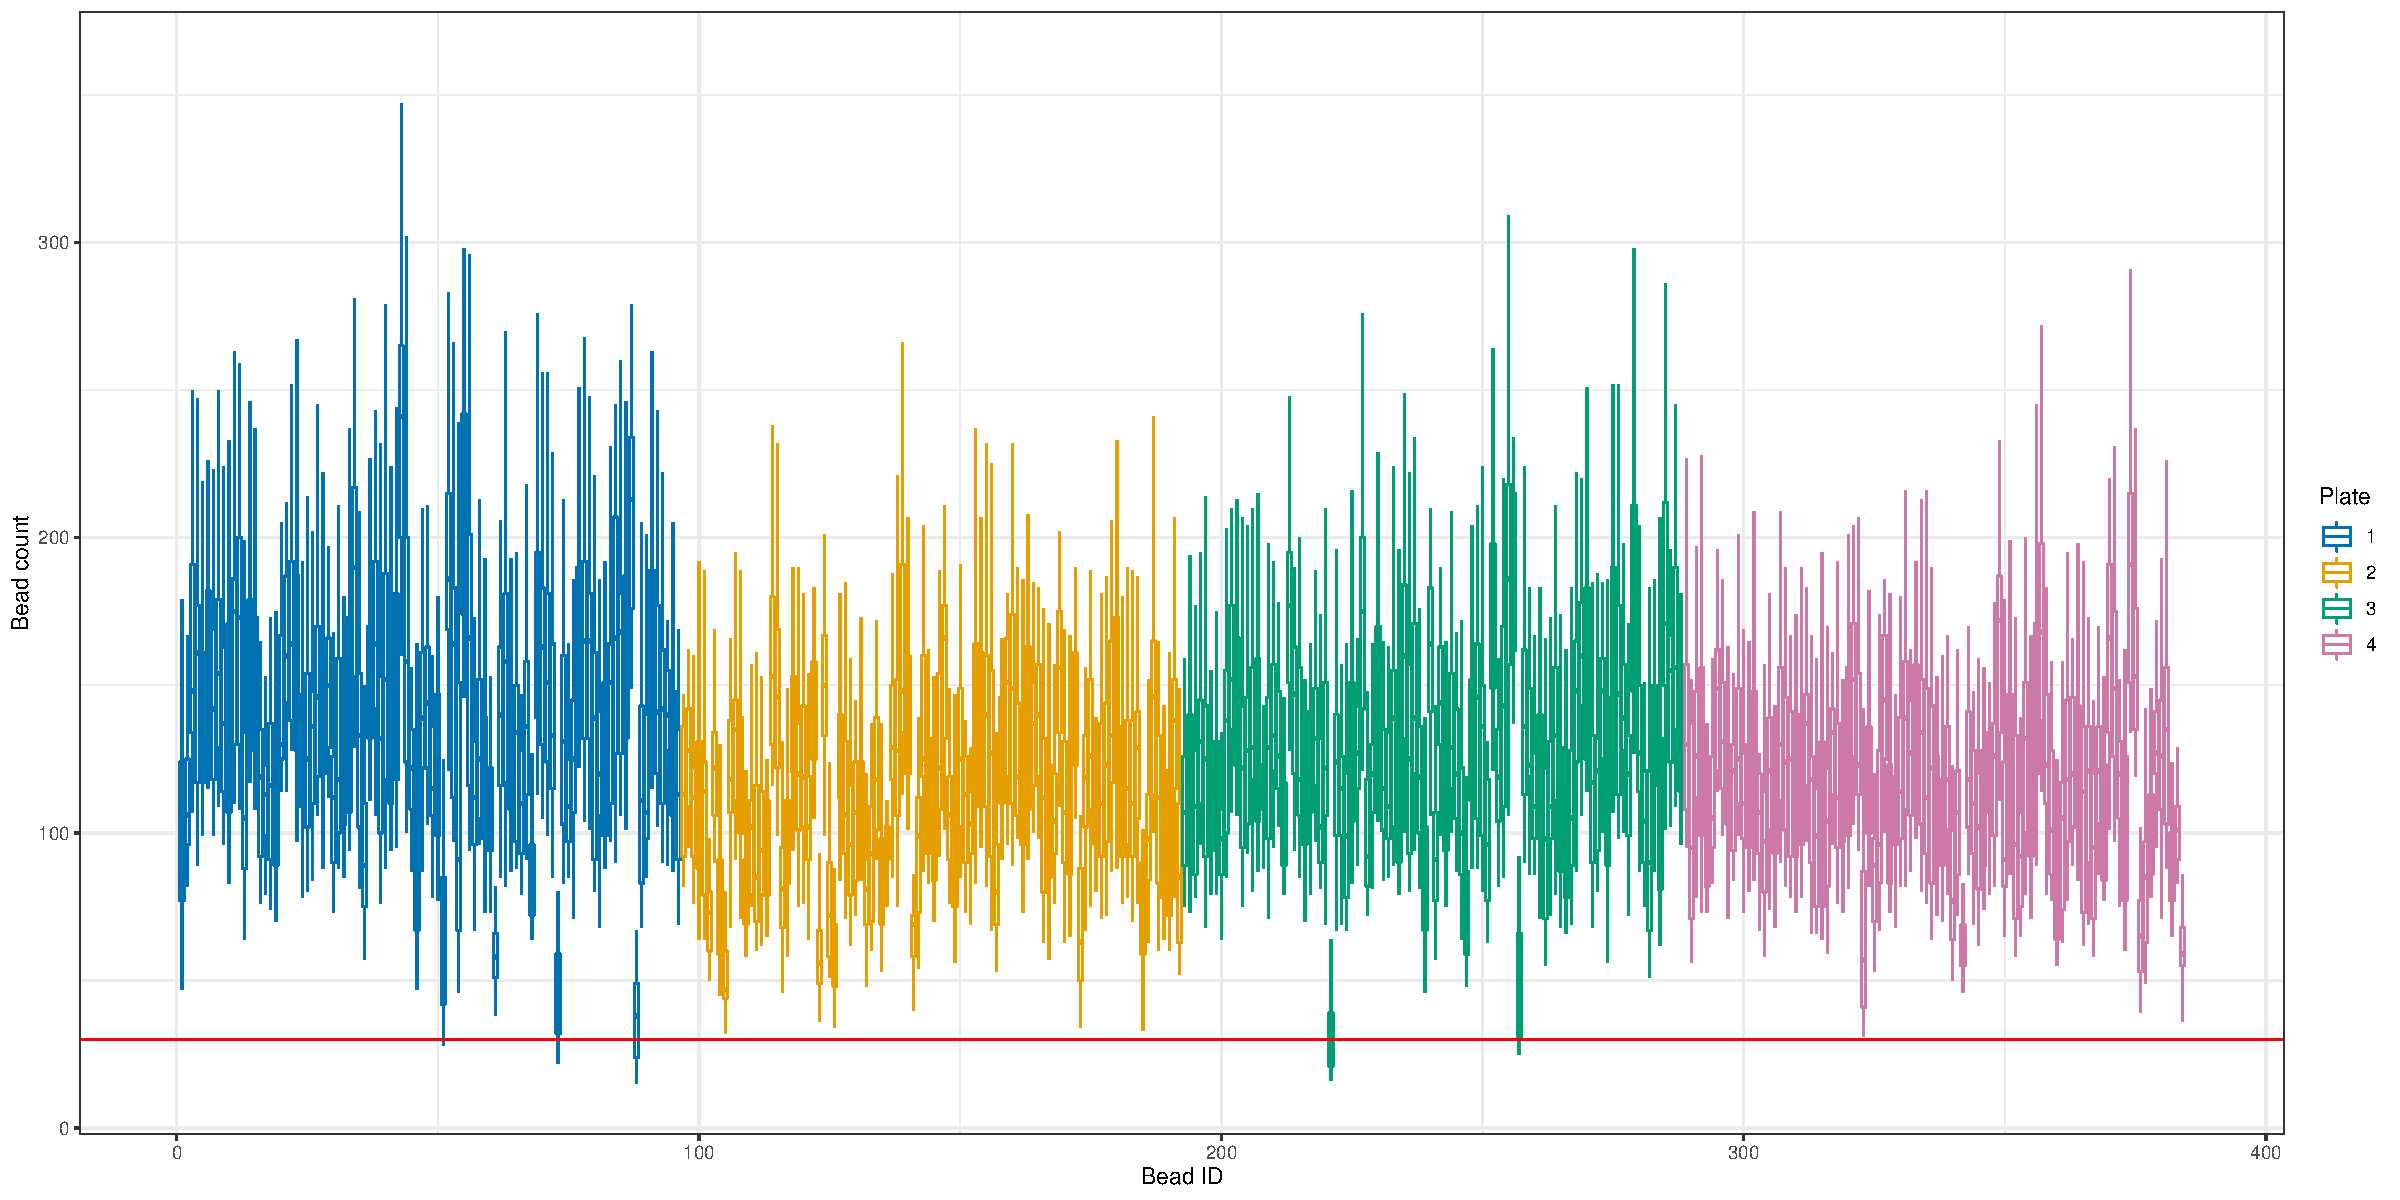
\includegraphics[width=0.8\linewidth]{figures/count_384.pdf}
	\caption{Boxplots consisting of the 21 observations of bead count across all bead IDs, color-separated by plate. The red horizontal line thresholds a bead count of 30.}
	\label{count_384}
\end{figure}

\newpage
The results of the coupling test are shown in figure \ref{fig_coupling_test}. As expected, the His$_6$ABP beads exhibits a high signal while the remaining control beads and non-PrEST antigen exhibit a low signal. The high variation in signal strength across the PrEST antigen can be due to variations in antigen coupling efficacy, but also due to varying tag accessibility across the PrESTs.

\begin{figure}[H]
	\centering
	\hspace*{2mm}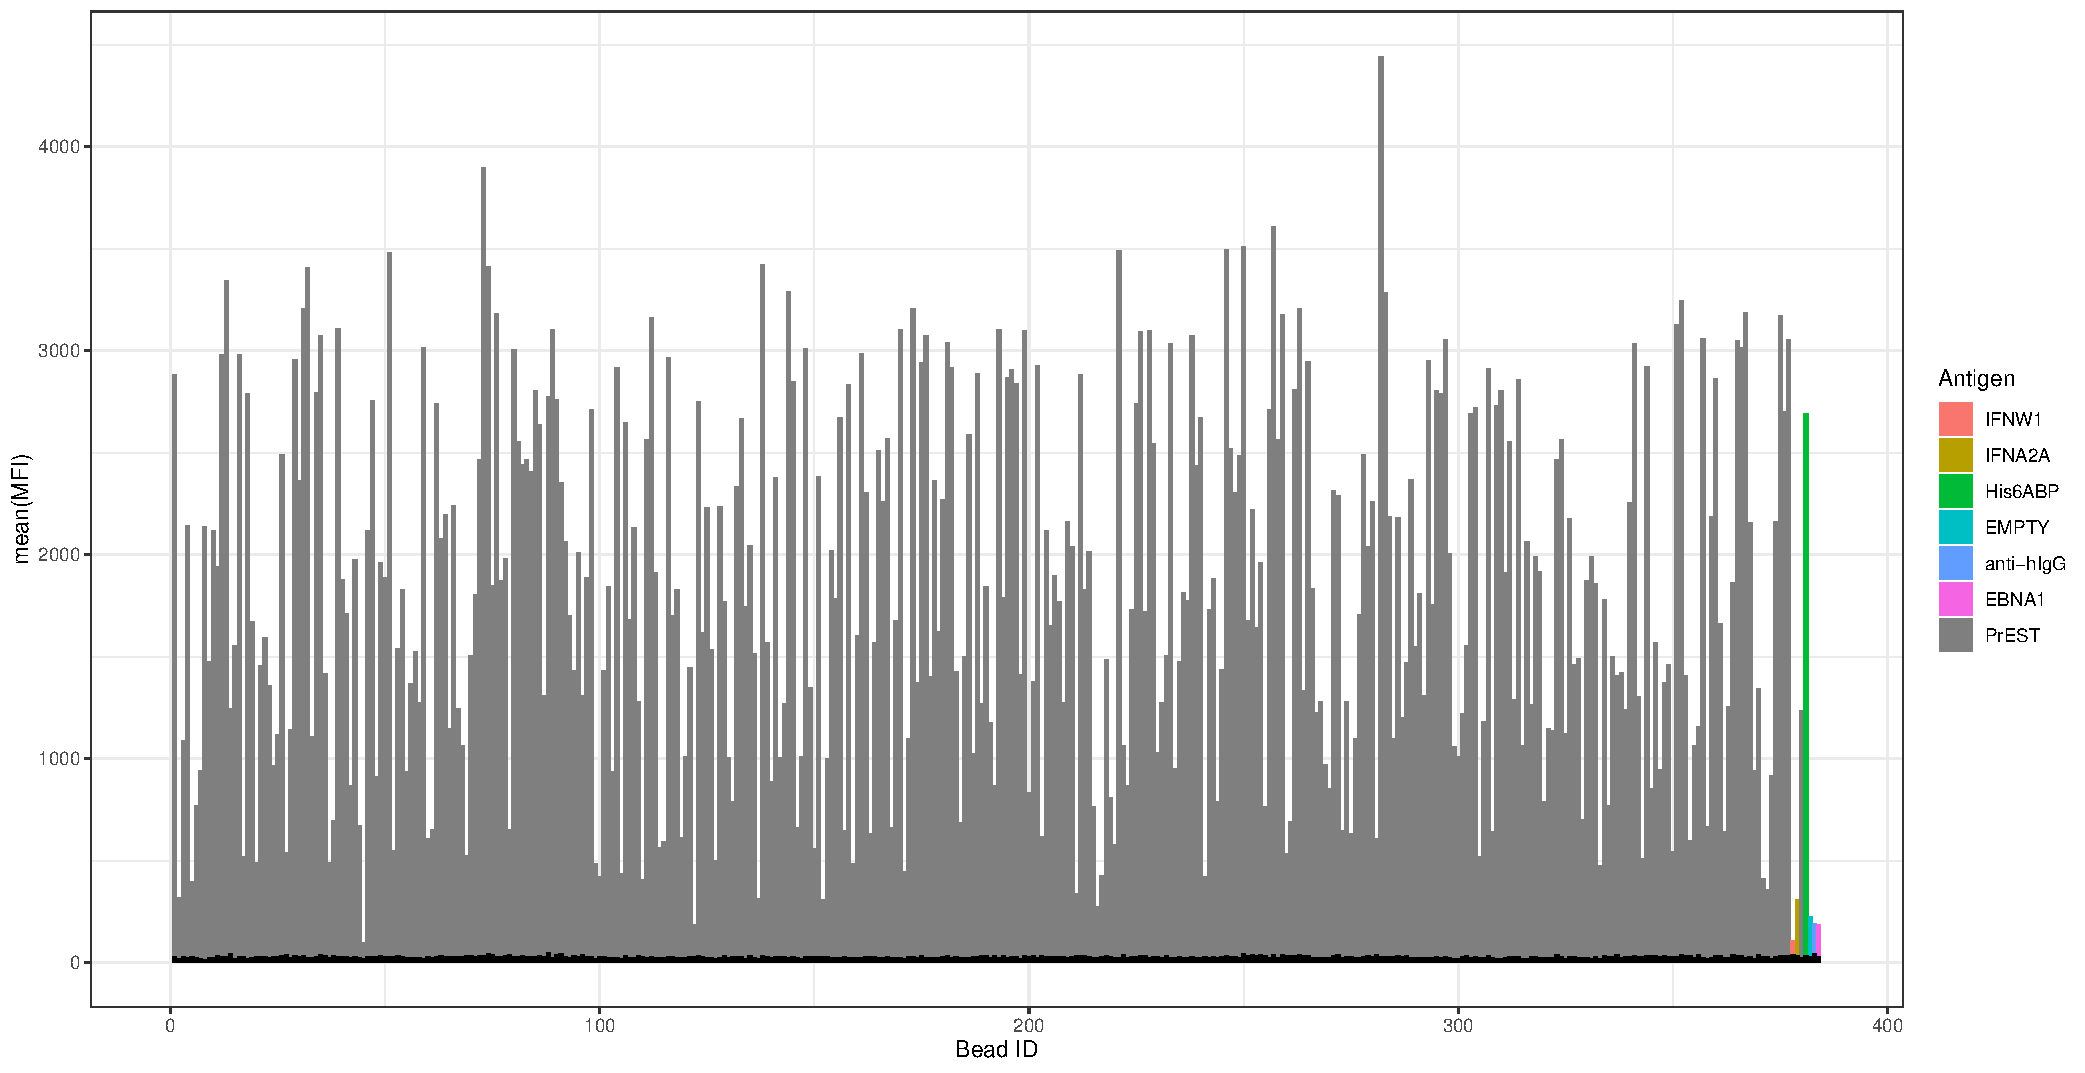
\includegraphics[width=\linewidth]{figures/coupling.pdf}
	\caption{The mean MFI of all bead IDs in the coupling test. The profile of the negative control is plotted in black in the foreground. All control beads as well as antigen without a His$_6$ABP tag are shown in bright colors.}
	\label{fig_coupling_test}
\end{figure}

The results of the sample test are shown in figure \ref{fig_sample_test}. The triplicate of commercial plasma has a limited number of reactivities across the antigen and a high reactivity for the anti-hIgG and EBNA1 beads as expected. The negative control is very low across all beads except anti-hIgG, were it amounts to around a third of the signal of the plasma triplicate.

The results of the specific antigen test are shown in figure \ref{specifig}. All HPA antibodies appear to have found their intended target PrESTs. Additionally, the full length protein IFN\textomega{} appears strongly reactive for the antibody targeting bead 89 (IFN\textomega) and weakly reactive for the antibody targeting bead 32 (various IFN\textalpha{} and IFN\textomega{}). The full length protein IFN\textalpha2A exhibits a very slight reactivity for the antibody targeting beads 33 (various IFN\textalpha) and is near indiscernible to the background for bead 32.

An unwanted, relatively low but consistent signal for anti-hIgG is seen across the negative controls of the sample test and specific antigen test which may be due to unspecific binding of the detection antibodies or contamination. All-in-all, the test results were seen as promising and no alterations were made to the array.

\begin{figure}[H]
	\centering
	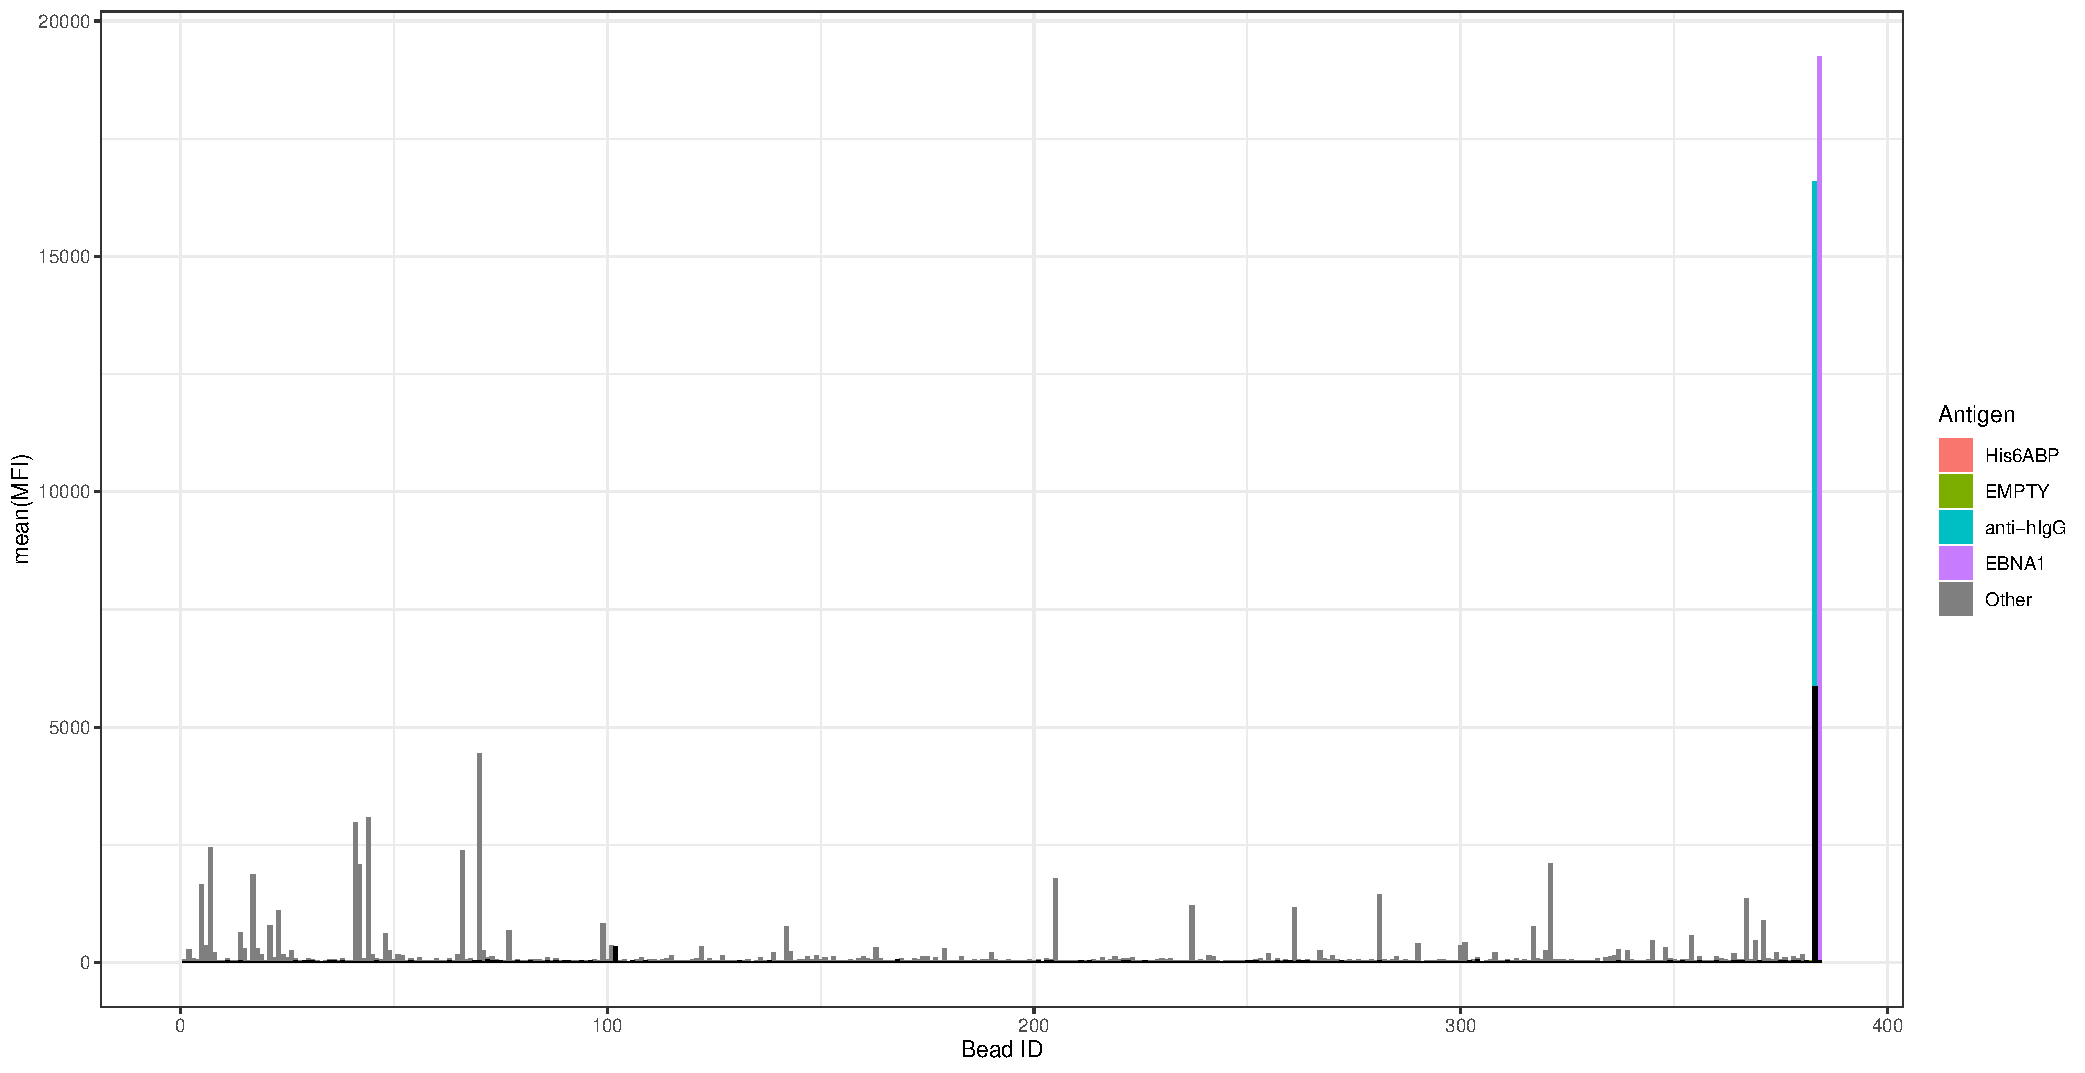
\includegraphics[width=\linewidth]{figures/sample.pdf}
	\caption{The mean MFI of all bead IDs in the sample test. The profile of the negative control is plotted in black in the foreground. All control beads are shown in bright colors.}
	\label{fig_sample_test}
\end{figure}
\begin{figure}[H]
	\centering
	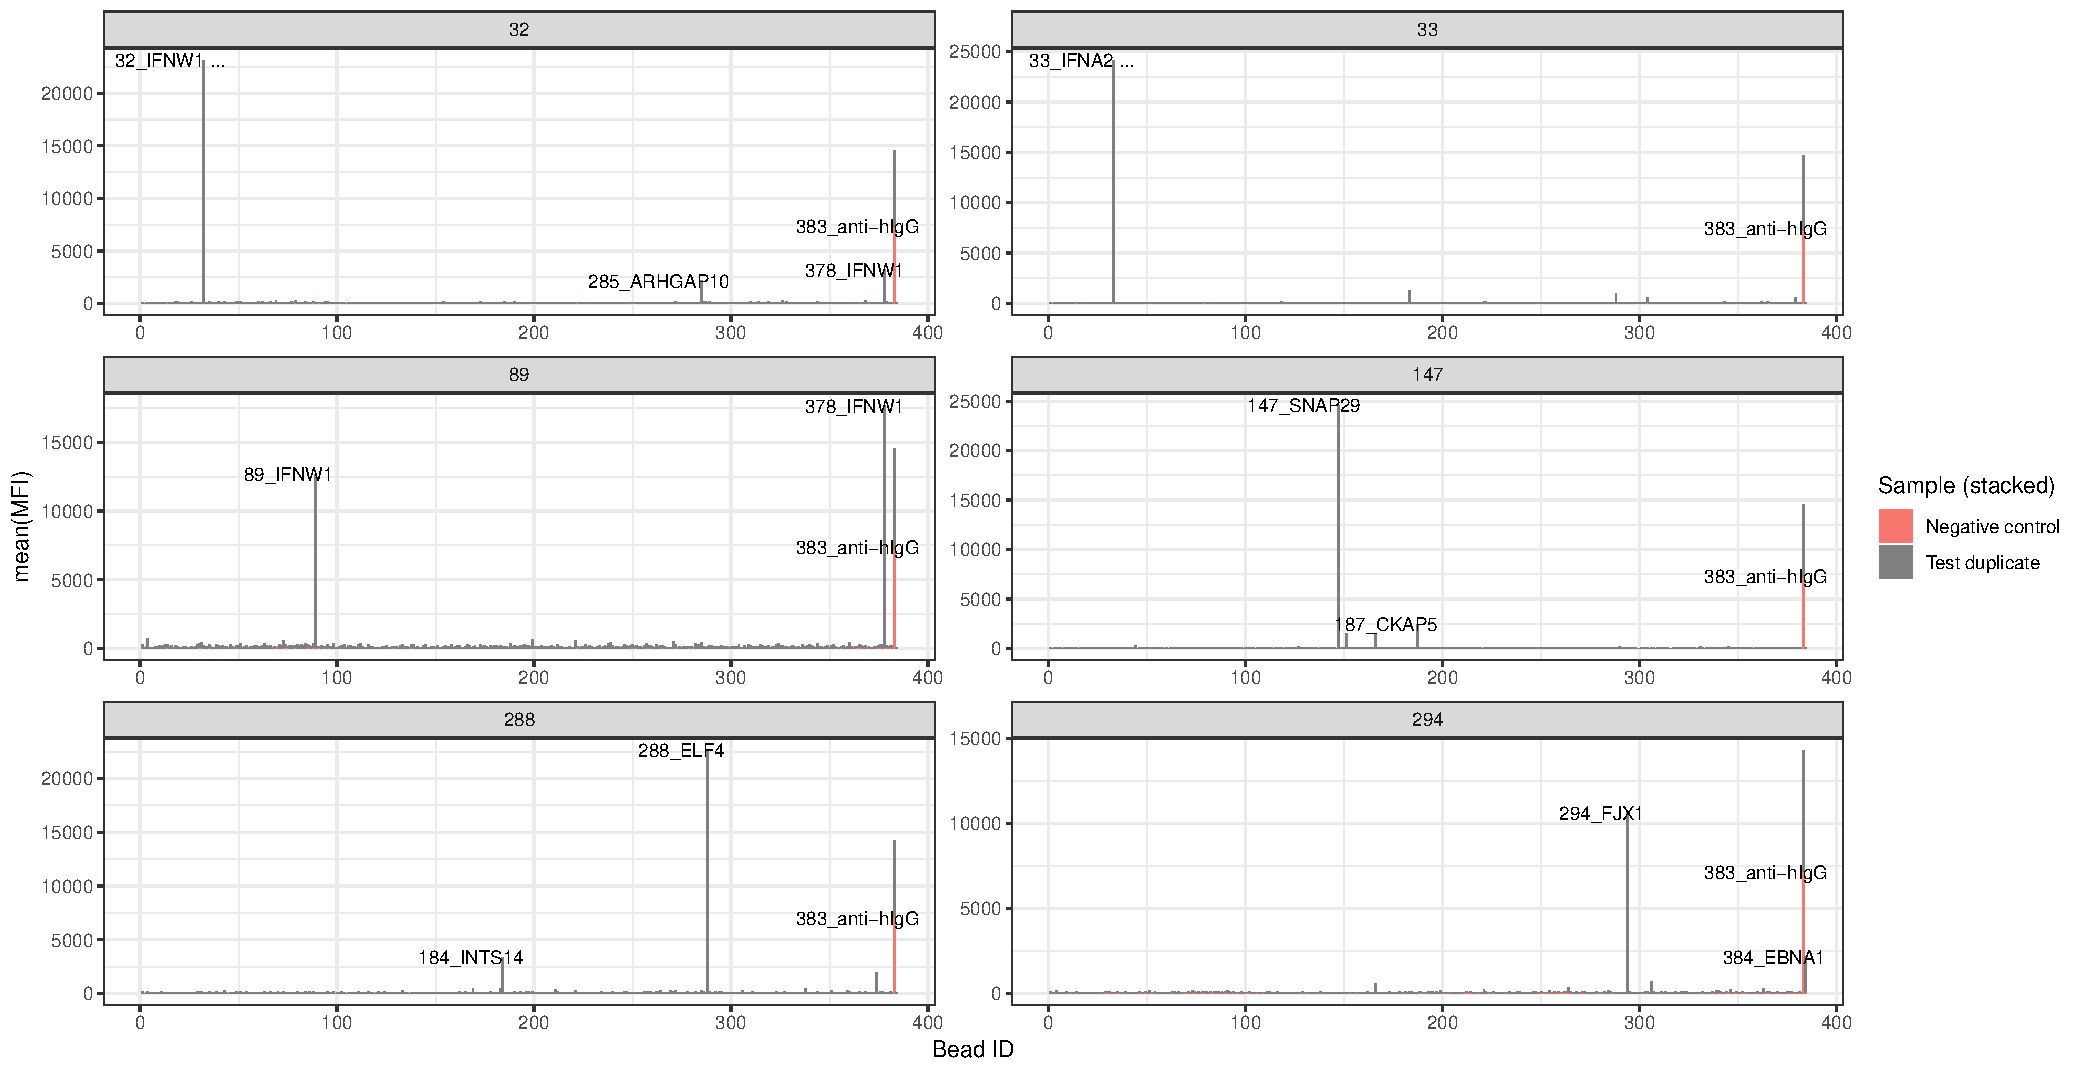
\includegraphics[width=\linewidth]{figures/specific.pdf}
	\caption{The mean MFI of all bead IDs, plotted for each of the six specific antigen tests, denoted by target bead ID. Outlier signals are captioned by bead ID and gene name. The columns of the negative control and antibody sample duplicates are stacked and shown in red and grey respectively.}
	\label{specifig}
\end{figure}

\newpage
\subsubsection{Quality control}
As can be seen in figure \ref{fig_control_beads}, the anti-hIgG bead indicates the binding of human IgG at uniform intensity across all non-empty wells. The EBNA1 bead exhibits a highly varying range of binding across all non-empty wells, but is more uniform for the commercial plasma and slightly lower in range for the Covid samples of phase 2 and 3. Both the empty bead and the His$_6$ABP appear inert across all wells.

\begin{figure}[H]
	\centering
	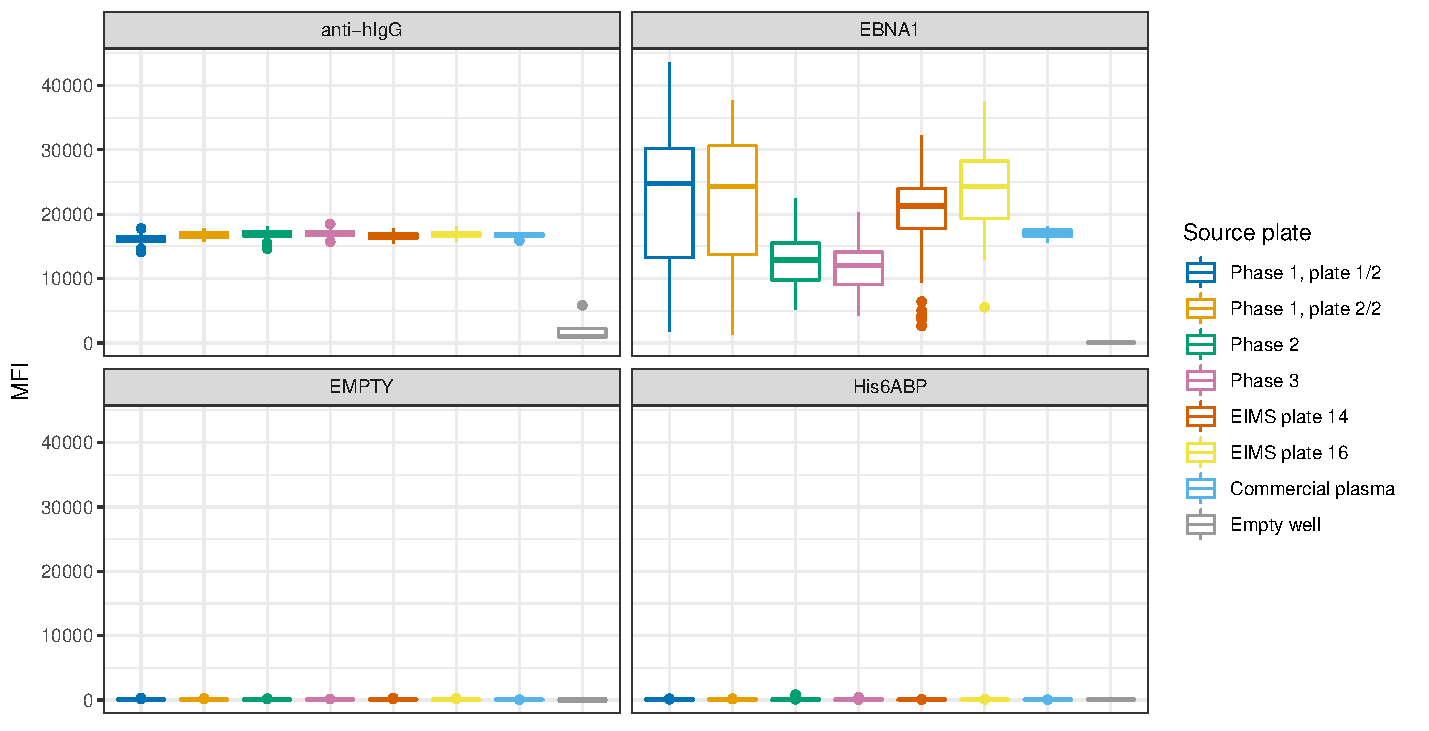
\includegraphics[width=\linewidth]{figures/control_beads.pdf}
	\caption{For all control beads (described in section \ref{method_control_beads}), the MFI is shown as a boxplot for each source plate as well as the commersial plasma controls and empty wells.}
	\label{fig_control_beads}
\end{figure}

\newpage
\subsubsection{Normal- and binarization}\label{res_norm}
In figure \ref{reactive_hist}, histograms of the number of reactivities per sample sample and antigen are plotted to provide an overview of the strictness of the set threshold. With medians of 12 reactive antigens per sample and 11 reactive samples per antigen, the chosen threshold does not contradict the assumption of the normalization (see \ref{statrat}).

\begin{figure}[H]
	\centering
	\begin{subfigure}[H]{0.8\linewidth}
		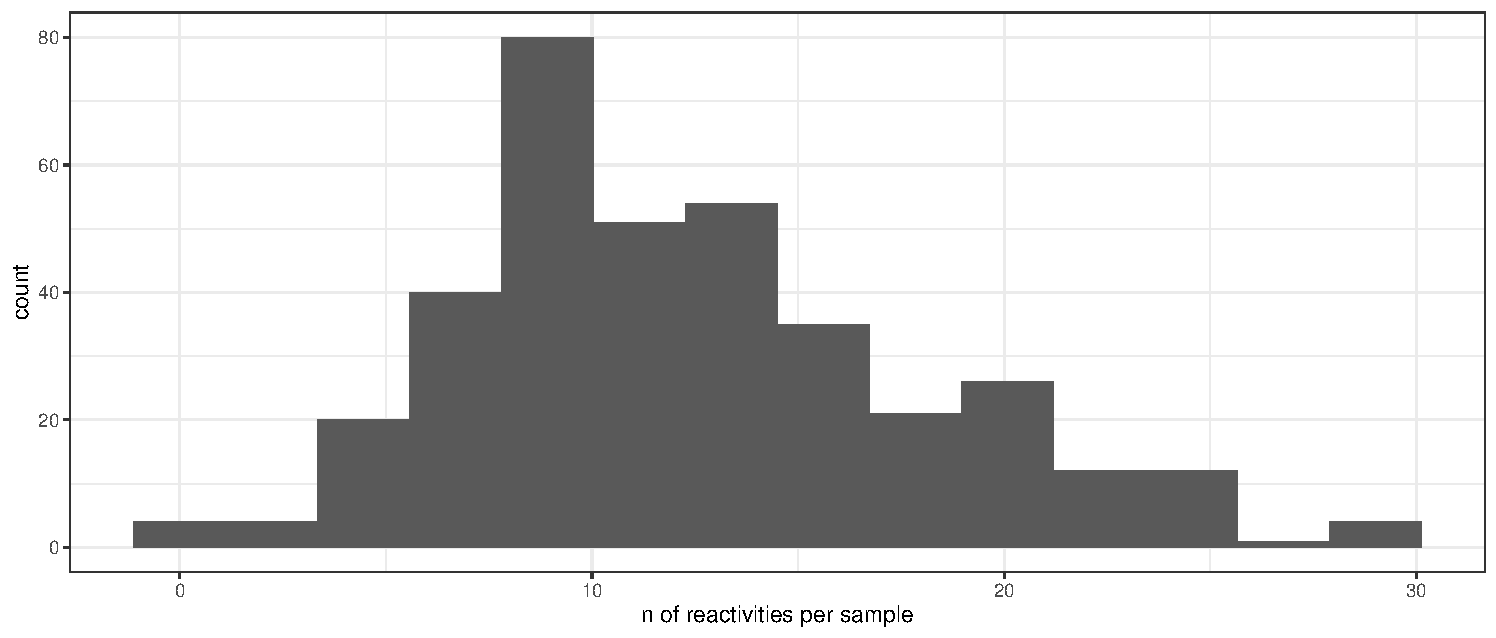
\includegraphics[width=\linewidth]{figures/reactive_per_sample.pdf}
	\end{subfigure}
	\begin{subfigure}[H]{0.8\linewidth}
		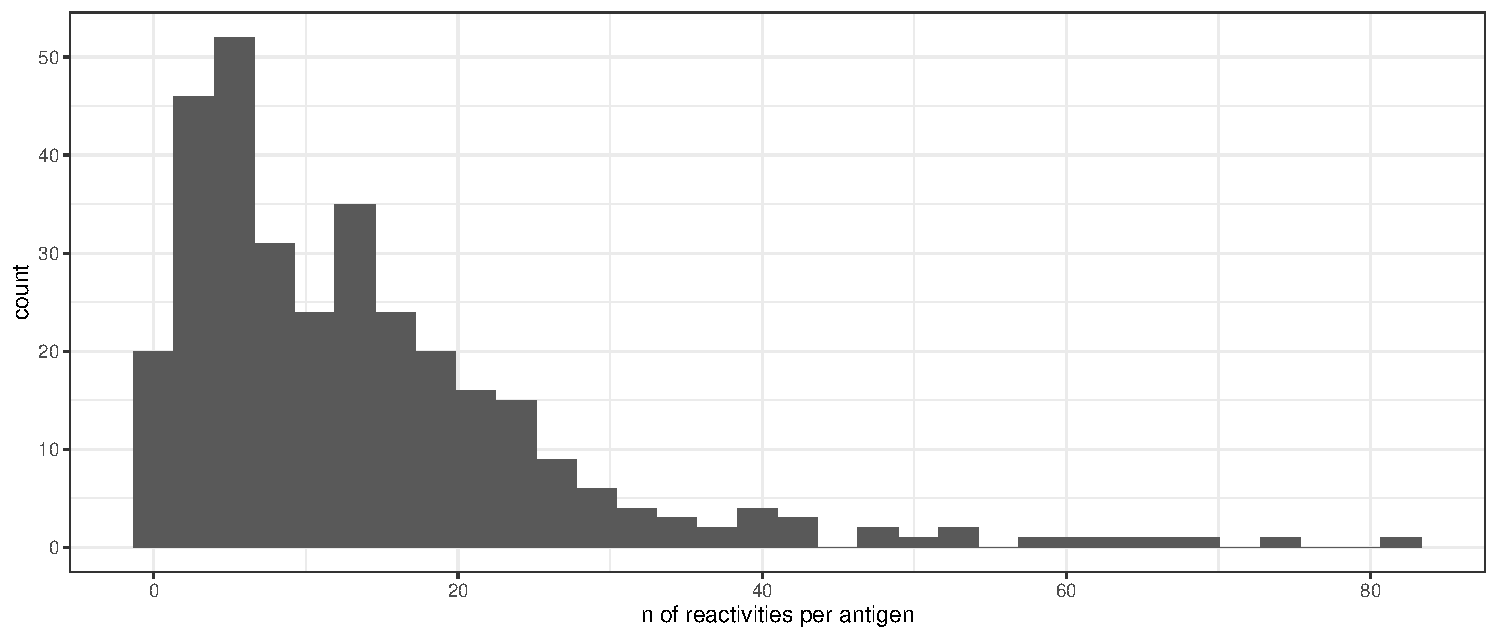
\includegraphics[width=\linewidth]{figures/reactive_per_ag.pdf}
	\end{subfigure}
	\caption{Histograms showing the number of called reactivities per sample (top) and per antigen (bottom).}
	\label{reactive_hist}
\end{figure}

Figure \ref{mfi2mads} shows the impact of normalizing each observation by the background of both it's sample and antigen. It is apparent that the transformation favors observations with relatively low backgrounds. For example, the PrEST with bead ID 5 representing the gene product RIN3 has a very high background compared to other antigens, but after transformation only a single observation is called as reactive. In contrast, the PrEST with bead ID 3 representing the gene product IL6 is appears to have it's signal range amplified in relation to the other antigens, due to low sample- and antigen background. It is worth noting that observations called as "reactive" are not claimed to possess any particular affinity or chemical property, merely that they are outliers in the normalized data. The threshold of 1.5 $MADs^{S,Ag}$ is above any observation in the negative control beads.

\begin{figure}[H]
	\centering
	\begin{subfigure}[H]{\linewidth}
		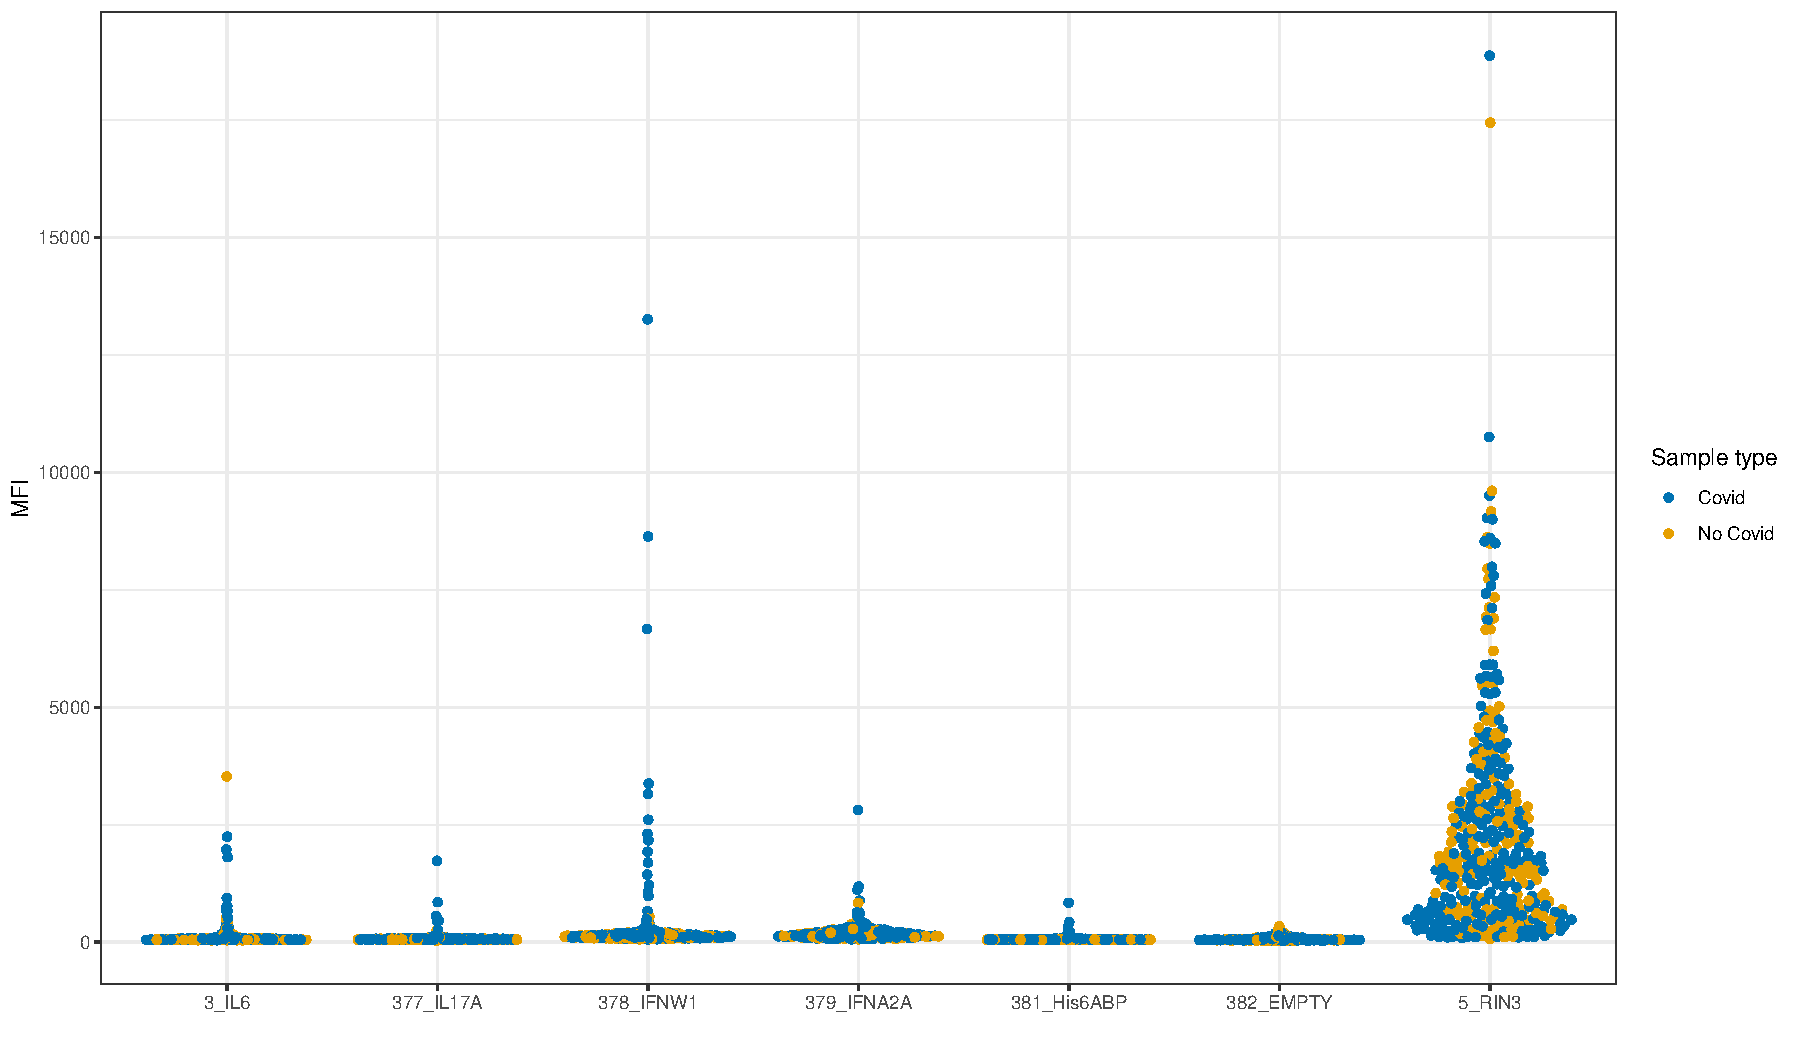
\includegraphics[width=\linewidth]{figures/norm_mfi.pdf}
	\end{subfigure}
	\begin{subfigure}[H]{\linewidth}
		\hspace{2mm}
		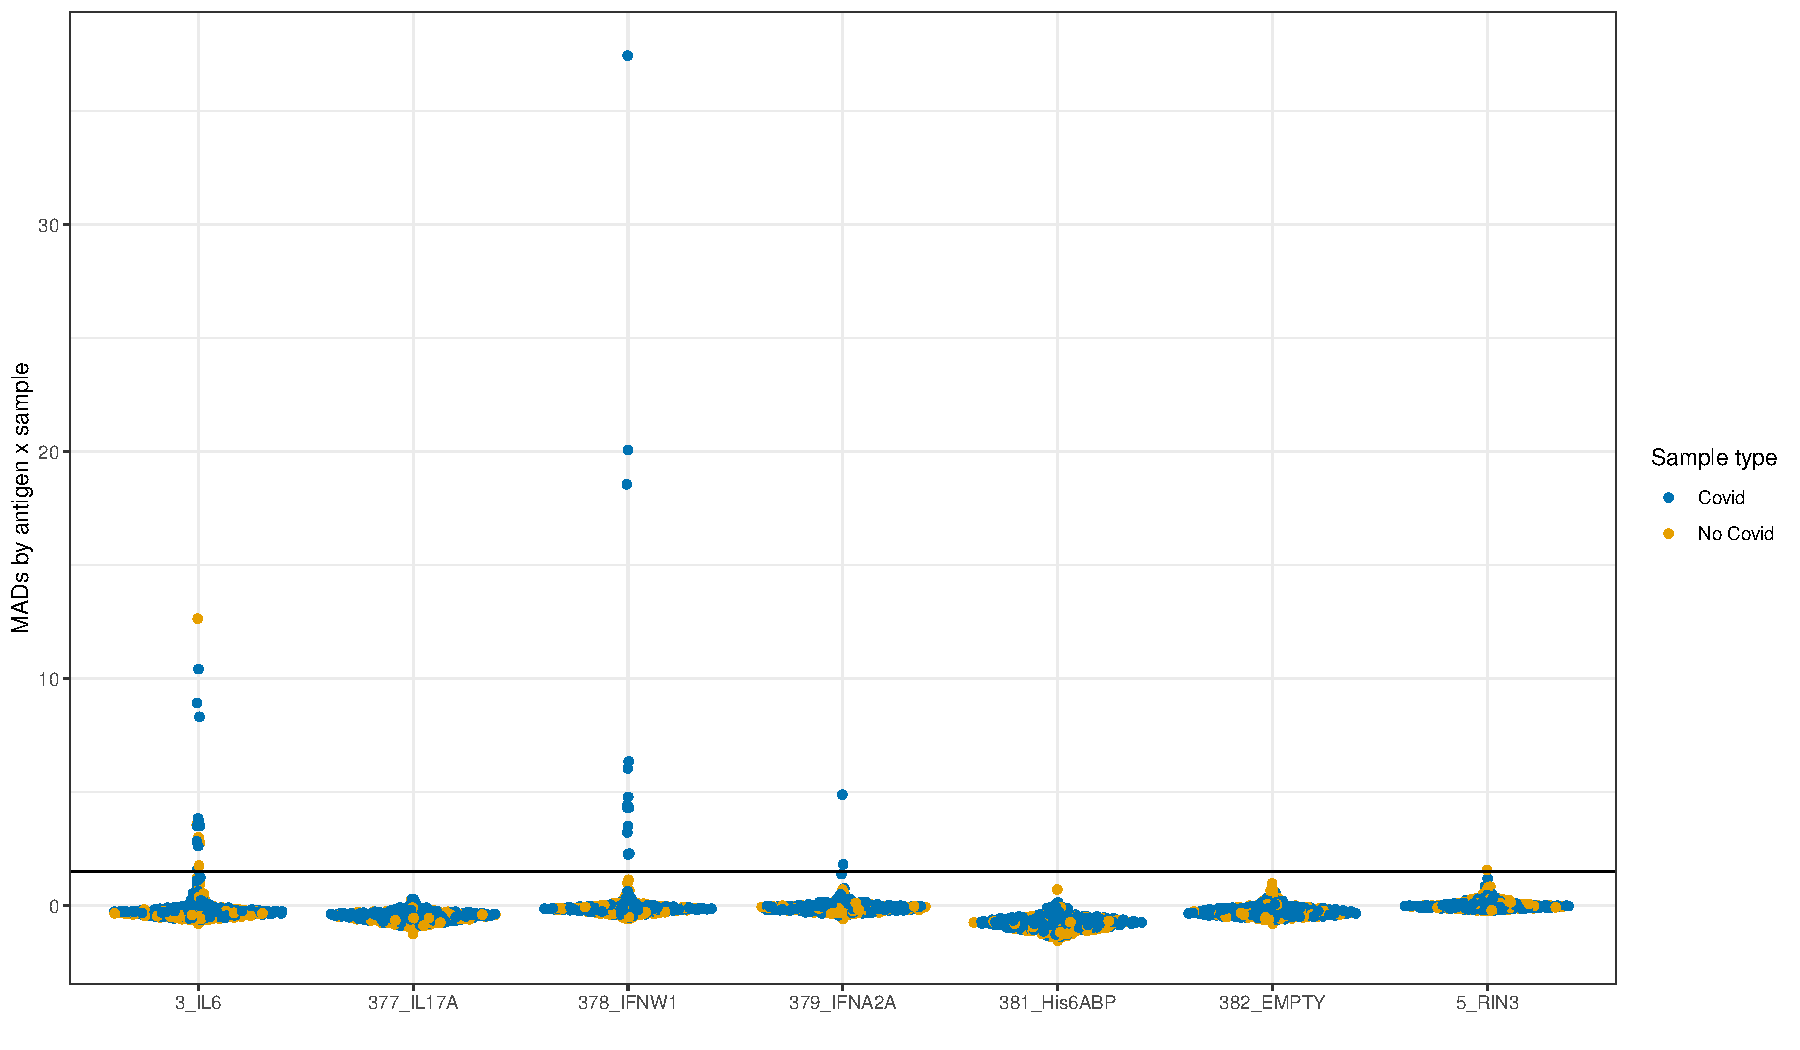
\includegraphics[width=0.98\linewidth]{figures/norm_mads2.pdf}
	\end{subfigure}
	\caption{Normalization of some example antigens. The bead ID and antigen name are shown sequentially on the x-axis. On the y-axis, the signal is shown in MFI (top) and normalized against sample and antigen backgrounds as described in equation \ref{2mads} (bottom). In the bottom plot, the horizontal line represents a cut-off of 1.5 $MADs^{S,Ag}$.}
	\label{mfi2mads}
\end{figure}

\subsubsection{Group comparison}\label{res_group_comp}
The complete results including p-values and contingency table values for each antigen and phase can be found in appendix \ref{full_group_res}.

In total, 34 antigen were called as differentially reactive in at least one phase. In the comparison between the Covid patients of phase 1 (n = 114) and the EIMS controls (n = 138), 21 antigens were found to be differentially reactive (p < 0.05). From phase 2 (n = 59) and 3 (n = 51), a total of 13 antigens were found to be differentially reactive but only 2 of these had seen a significant increase in the number of reactive patients. 

To provide some structure and prioritization among the results, the antigens were divided into three categories:

\begin{itemize}
    \item \textbf{Excluded (n = 11)} Because the Covid patient samples of phase 2 and 3 are sub-cohorts of phase 1, their sample sizes are smaller. This means significance may be lost in phase 2-3 because the reactive patients did not participate in the follow up. It also means significance may be gained in phase 2 or 3 simply because the sample size has decreased, affecting the proportion of reactive patients. For this reason, antigens which reached significance in phase 2 or 3 but had not increased considerably in number of reactive patients since phase 1 were excluded from the results and are not discussed further.
    
    \item \textbf{Relevant (n = 8)} Antigens with immunoregulatory properties and/or particular perceived relevance to Covid pathogenesis, based on literature and gene ontology.
    
    \item \textbf{Various (n = 15)} Remaining antigens, which may still be of importance but will not be prioritized in the results or discussion to limit the scope of this project.
\end{itemize}

In figure \ref{gucci_relevant}, all observations of the antigens classed as relevant are visualized by antigen, phase, signal, reactivity and subject. The same plots can be found for the remaining various antigens in appendix \ref{gucci_various}. Note that the signal ranges differ between antigens, but that they are scaled individually to better visualize their distributions.

\begin{figure}[H]
	\centering
    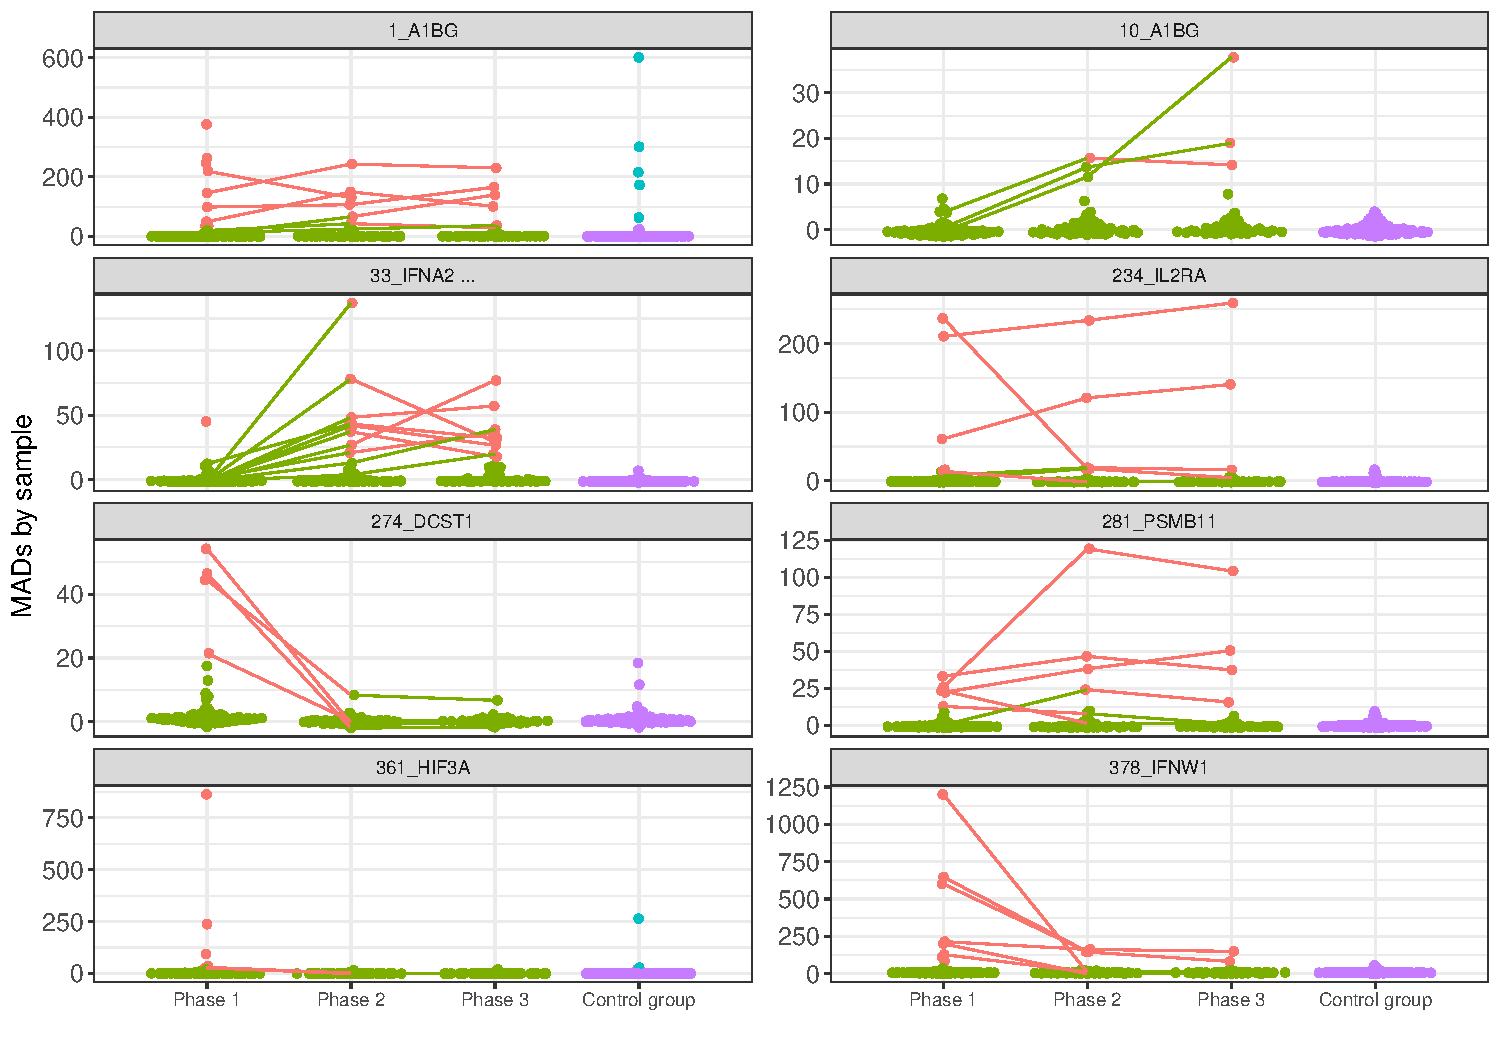
\includegraphics[width=\linewidth]{figures/gucci_relevant.pdf}
	\caption{Swarm plots of all differentially reactive antigens classed as relevant. The x-axis is divided into all three phases of the Covid cohort as well as the control group. The y-axis shows the sample-normalized signal ($MADs^S$) scaled per antigen. Reactive and non-reactive observations are colored for the Covid patients (red, green) and control samples (blue, purple) respectively. Observations of patients who were reactive in at least one phase are interconnected, to visualize which patients did not participate in follow-up and how the reactivities of the same individuals change longitudinally.}
	\label{gucci_relevant}
\end{figure}

The results of these antigens are briefly summarized below:

\begin{itemize}
    \item Beads 1 and 10 both represent different epitopes of Alpha-1B-glycoprotein. Immunologically, the protein is involved in neutrophil degranulation which plays part in Covid pathogenesis and lung tissue damage \cite{neutrophil_damage}. In phase 1, bead 1 is reactive in 13/114 Covid patients compared to 5/138 controls and the number of reactivities decreases in phase 2-3 due to patient fall-off. Bead 10 on the other hand increases longitudinally in 3 patients compared to no controls. The PrEST of bead 1 is "sticky" with a high background and found reactive in ~31\% of in-house runs while that of bead 10 is not. 
    
    \item For most antigens, the number of reactive patients generally decreases in phases 2-3. The most notable exception is bead 33 representing 12 subtypes of IFN\textalpha{} which increases from 1 to 9 reactive patients longitudinally (1 to 11 when including reactive patient fall-off). This corresponds to 17.6\% of phase 3 or 7.9\% of phase 1 patients exhibiting reactive levels of anti-type I IFN aAbs 8 months after infection, compared to none in the control group. 
    
    \item Bead 234 represents the Interleukin-2 receptor subunit alpha which is reactive in the same 5 Covid patients across phases 1-2, after which 2 drop below the reactivity threshold in phase 3. The interleukin-2 receptor enables T-cell differentiation into regulatory T-cells, as well as effector T-cells and memory T-cells, upon antigen binding, to combat infections \cite{il2ra}.
    
    \item Bead 274 representing E3 ubiquitin-protein ligase is reactive in 4 Covid patients in phase 1 of which all drop below the reactivity threshold in phase 2-3. The protein is a negative regulator of type I interferon-mediated signaling and plays part in the innate immune response \cite{GO}.
    
    \item Bead 281 representing Proteasome subunit beta type-11 is reactive in 5 Covid patients in phase 1 after which two drop and another is gained in phase 2-3. The protein is a part of the proteasome which is responsible for antigen processing and presentation via MHC class I during viral infection \cite{GO}.
    
    \item Bead 361 representing Hypoxia-inducible factor 3-alpha is called reactive in 8 Covid patients (although only 3 are visible above the bulk) in phase 1 compared to 2 controls, after which one patient goes below the reactivity threshold and the remaining seven fall off in phase 2-3. Some called reactivities here are admittedly close to the background, but one Covid patient exhibits a very high signal in phase 1. The protein is a transcription factor which regulates the transcriptional response to low oxygen tension \cite{hif}, a hallmark symptom and pathological element in Covid-19.
    
    \item The full length protein IFN\textomega{} has the 5\textsuperscript{th} highest signal range of any differentially reactive antigen and the highest among the antigens classed as relevant. In phase 1, 8/114 patients (7\%) were classed as reactive compared to none in the control group, after which 3 and 2 remain reactive in phase 2 and 3 respectively.
\end{itemize}

All of the relevant antigens except HIF3A have an immunological or immunoregulatory function and all except PSMB11 are extracellularly accessible. Of the 15 various antigens, 2 are annotated to have minor immunological functions and 7 are extracellularly accessible (see appendix \ref{full_group_res}).

Among the Covid patients who had participated in both phase 1 and 2 (n = 59), 194 out of 687 (28.2\%) observed reactivities decreased past the reactivity threshold in phase 2. In comparison, only 334 out of 21,662 (1.5\%) of non-reactive observations did the opposite transition of increasing past the reactivity threshold.

\subsubsection{Type I Interferons}
In the interest of comparing the results to the findings of of Bastard \textit{et al}, it is worth mentioning the outcome of the beads representing type I IFNs. There were 11 such beads included in the panel: 2 were called as differentially reactive (mentioned above) and another 4 had at least one Covid patient classed as reactive in some phase. They are shown in figure \ref{gucci_ifn}. For each of these antigen, including the full length IFN\textalpha2A, only a few patients were reactive, albeit often with clear and consistent signal across the phases. The remaining 5 beads (ID 31,73,89,141,239) were not classed as reactive in any observation.

\begin{figure}[H]
	\centering
    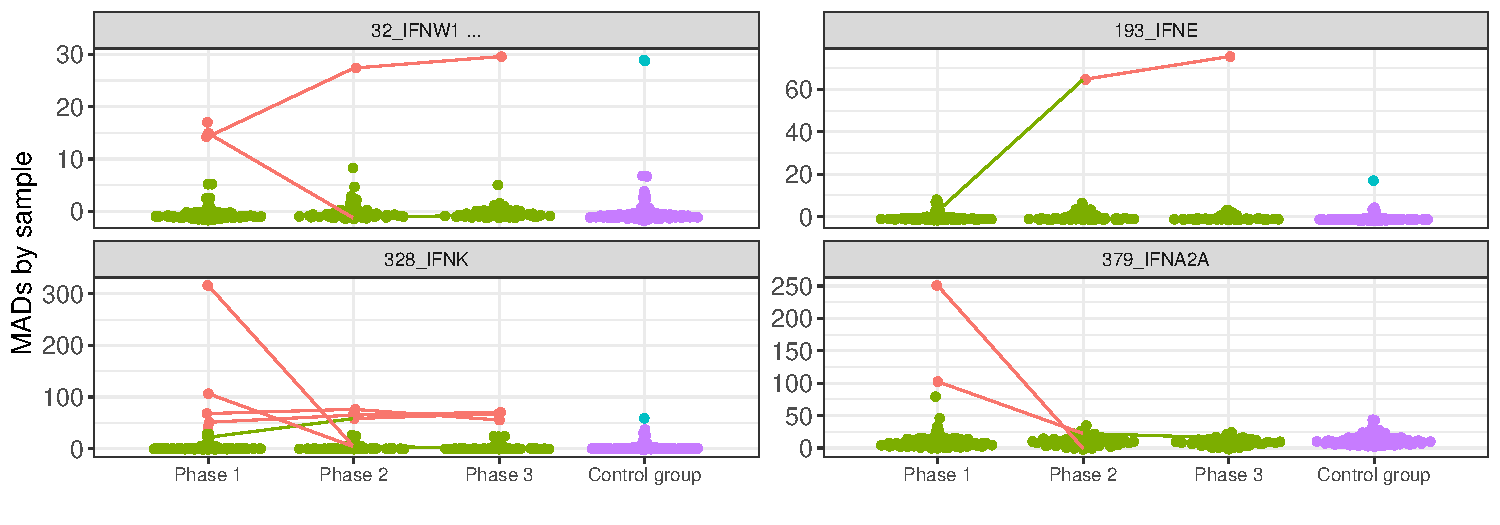
\includegraphics[width=\linewidth]{figures/gucci_other_ifn.pdf}
	\caption{Swarm plots of beads representing type I IFNs which were reactive in at least one phase but not classed as differentially reactive. The x-axis is divided into all three phases of the Covid cohort as well as the control group. The y-axis shows the sample-normalized signal ($MADs^S$) scaled per antigen. Reactive and non-reactive observations are colored for the Covid patients (red, green) and control samples (blue, purple) respectively. Observations of patients who were reactive in at least one phase are interconnected, to visualize which patients did not participate in follow-up and how the reactivities of the same individuals change longitudinally.}
	\label{gucci_ifn}
\end{figure}

\addtocontents{toc}{\protect\newpage}
\section{Discussion}
\subsection{Findings}
\subsubsection{Candidate autoantigens}
In total, 23 candidate autoantigens were called as differentially reactive in Covid patients, of which 8 were identified as biologically relevant to immunoregulation and/or Covid pathogenesis.

Due to the low sample size and exploratory nature of the project, no definite conclusions can be drawn solely based on these results. However, the results can be put in relation to previous findings and may be useful for future investigations of the interplay between Covid-19 and autoimmunity phenomena.

\subsubsection{Type I interferons and previous findings}
Based on the findings of Bastard \textit{et al}, autoantibodies directed towards IFN\textalpha2 and/or IFN\textomega{} were expected in ~10\% of hospitalized patients (n = 101/987). In this project, 8/114 (7\%) of hospitalized patients were reactive to full length IFN\textomega{} which is arguably well in line with the findings. Surprisingly however, only 2/114 (1.8\%) were reactive to the full length IFN\textalpha{} which is described as the more common reactivity of the two. 

Out of the four PrESTs representing epitopes of IFN\textalpha/\textomega, two (beads 31 and 89) were not called as reactive at any point and one (bead 32) was called as reactive in 3 Covid patients compared to 1 control. Lastly, bead 33 representing a common type I interferon epitope exhibited the single highest significance of any antigen at 9/51 (17.6\%) reactive patients in phase 3 compared to no controls. As shown among the Covid patients, reactivities are much more commonly lost than gained after phase 1, which may indicate an elevated general presence of antibodies during hospitalization which later rescinds to baseline. This trend is contradicted by bead 33: out of all differentially reactive antigens, it is the only one to consistently increase in number of reactive patients throughout the 8 month period.

Whether this increase of autoantibodies is novel and contracted due to the Covid infection is not known as there is no data regarding the autoantibody levels prior to infection. It can be speculated that the autoantibody response of these patients were present before and during phase 1, but that the circulating autoantibodies were depleted by high levels of antigen \textit{in vivo} during the course of the disease.

Some reactivities were observed in the Covid patients for PrESTs representing other type I interferons such as IFN\textepsilon{} and IFN$\kappa$, yet the significance of the findings are limited primarily by sample size.

\subsubsection{Differences between PrESTs and full length proteins}\label{disc_diff}
The inclusion of the full length proteins in the SBA offers the opportunity to compare their reactivity to that of the PrESTs. Several beads representing IFN\textalpha/\textomega{} were called as completely inert, and most were less reactive than the full length IFN\textomega{}. This indicates that the PrESTs on these beads do not fully present the antigenic epitopes of the full length protein, possibly due to the epitopes in question being conformational in nature or simply situated in a sequence-part of the protein which is not represented. Intuitively, it makes sense that the reactivities of the PrESTs would constitute a subset of the reactivities towards the full length proteins, because they exhibit a subset of the epitopes.

On the other hand, bead 33 demonstrated both a higher number of reactivities and a completely inverted longitudinal profile compared to both full length proteins. In this case, it could be speculated that the PrEST does present a reactive epitope as well as being more accessible to binding due to a smaller size and an increased conformational freedom.

As was apparent in the specific antigen test and figure \ref{specifig}, antibodies which were specifically derived from PrESTs may not bind the full length protein strongly. The HPA antibody of bead 89 representing IFN\textomega{} did bind to both the PrEST and the full length protein, yet the bead was called as completely inert to the antibodies of the samples, that instead bound other representations of IFN\textomega. This suggests that even epitopes that are accessible on the full length proteins are not necessarily immunogenic.

All in all, the results of this project indicate that PrESTs and full length proteins can be expected to differ in reactivity. The PrESTs may be less reactive than their mimicked proteins due to not being fully representative. On the other hand, using many PrESTs representing the same protein may provide a multi-faceted approach in which binding is evaluated for different epitope representations of different conformational freedoms which may partially compensate for the artifacts arising in an \textit{in vitro} approach. A combination approach of including both full-length proteins and their PrESTs may be beneficial in combining the advantages of both. 

\subsection{Limitations}
\subsubsection{The challenges of autoimmunity profiling}
Autoimmunity profiles are inherently diverse and scattered, and with a broad enough antigen panel even clinically healthy samples will exhibit some activity \cite{aa_healthy}. Because even significant autoreactivities may only be present in a relatively small proportion of patients, it may be difficult to determine overlaps and significant enrichments even in a sizeable cohort.

A further complication is that free antibody levels in the plasma may fluctuate over time depending on the state of the immune system and the availability of target antigen. In the results there are several examples of reactivities decreasing or increasing, as well as remaining stable, over time. Another challenging aspect is that these assays measure free antibodies, entailing that antibodies may be "depleted" to a varying extent depending on the level of target antigen in the plasma.

\subsubsection{Sample quality and quantity}\label{disc_sample}
The most limiting aspect of this project is arguably the sample size. When measuring autoimmunity present in less than 10\% of hospitalized Covid patients, even hundreds of samples may not provide statistically significant results. The relative rarity of autoimmune features also makes it difficult to make statistically sound investigations within the feature group, e.g. looking at the impact of sex and age. These parameters were also only available for the EIMS controls and the Covid patients of phase 2 and were not largely utilized in the analysis.

When looking for autoimmunity features impacting the severity of the disease in hospitalized patients, the direct comparison to mild Covid cases would have been more powerful than using a control group consisting of a combination of MS-patients and healthy controls with no known relation to the disease. The usage of the EIMS control group was primarily motivated by limited access to other samples. However, the frequency of Covid cases requiring hospitalization in the population at large is low and therefore the majority of the controls should arguably represent mild cases.

\subsubsection{Panel composition bias}
Out of the 380 antigen included in the panel, 353 are based on the planar microarray analysis of 16 patients and 27 are based on literature. Basing such a large fraction of the panel on such a small fraction of patients is optimistic, especially for autoimmunity profiling. This is because not all antigens which may be differentially reactive at group level can be expected to be captured in such a small sample size. It is important to clarify however, that the "pilot" group of 16 patients never was expected to fully and comprehensibly represent all Covid patients, but rather provide a list of possible autoantigens to further investigate at a group level. The pool-wise stratification by disease severity, sex and comorbidity of the pilot group was not largely utilized in the rest of the project, but the justification of minimizing comorbidities (see section \ref{method_42}) still applies.

The differentially reactive, non-excluded antigens (n = 23) consisted of 21 (91.3\%) microarray antigens and 2 (8.7\%) literature antigens compared to the panel at large (n = 380) which consisted of 353 (92.9\%) microarray antigens and 27/380 (7.1\%) literature antigens. In summary, antigens which were specifically motivated as relevant in literature were slightly enriched in the results.

\subsubsection{Cut-offs}
There are two important cut-offs set in the data analysis of this project and both largely affect the results.

The first is the cut-off for binarizing reactivity, set at 1.5 $MADs^{S,Ag}$. Normalizing all observations by both sample and antigen background in order to set a universal cut-off value is applicable for an assay containing a large number of samples and antigen, where the majority of both are nonreactive. Another, clinical approach is to use a negative control group to define the range at which a signal is deemed non-reactive for a particular antigen. This presumes certainty that the control group is wholly nonreactive towards the antigen in question, which is not applicable in this broad and discovery-based project. A more complex, data-driven approach is to analyze each antigen distribution separately with respect to the impact of different cut-offs on comparisons across the groups. The tools for such an approach were available, but were not applied in order to prioritize self reliant work and learning under a time constraint.

The method chosen for this project is justified in that it takes both sample and antigen backgrounds into consideration while still performing a relatively simple transformation. The threshold is fairly generous, set slightly above the distribution of the empty beads, but this generosity can be justified in that the end purpose is to compare the reactivity between the groups, rather than the reactivity within the groups. E.g. as long as the cut-off is equally generous for both groups in the comparison, the impact is small.

The second cut-off is for the p-value of Fisher's Exact Test, under which a finding is called significant. Statistically speaking, the SBA assay investigates 380 antigens in conjunction, corresponding to an equal number of alternative hypotheses to be tested. It can be argued that this warrants multiple hypothesis correction to compensate for the increased chance of erroneous significance calls. However, it can be argued that multiple hypothesis approaches, such as Bonferroni correction and False Discovery Rate (FDR), are more appropriate for quantitative comparisons in which the p-values fall in a mostly uniform distribution. Due to the contingency basis of Fisher's Exact Test (which in itself is a direct result of the binarization cut-off) and the relatively low sample size, the p-value distribution does not follow the assumption of the mostly uniform distribution on which many correction methods are based. Furthermore, the purpose of the significance cut-off in this exploratory project is not to draw statistically ensured conclusions but rather to arrange the results in order of interest.

\newpage
\section{Conclusion and future perspectives}
This project proposes several candidate autoantigens for which autoantibodies were found to be enriched in a subset of patients afflicted with severe Covid in a Swedish cohort. Out of the 23 differentially reactive antigens, 8 are motivated as biologically relevant to immunoregulation or Covid pathogenesis. Previous findings of cytokine-directed autoimmunity in Covid patients \cite{bastard} were replicated for full length IFN\textomega{} as well as a PrEST representing a common type I interferon epitope, with the former peaking in reactivity during the hospital admission and the latter increasing in reactivity over an 8 month period.

The results of this project further advance the notion of autoimmunity as an underlying risk factor of severe Covid and invite further investigation. As a suggestion, similar inquires may, in the future, benefit from a larger sample size and a qualitatively similar control group (discussed in section \ref{disc_sample}).  It is also worth noting that the scope of this project has been limited to detecting autoimmunity directed to proteins and protein fragments, while autoantibodies can be directed to other classes of biomolecules as well, such as phospholipids.

The variation of reactivity seen across the full length proteins and their respective PrESTs (discussed in section \ref{disc_diff}) indicate that neither approach captures all reactivities seen in the other, suggesting that a combination of full-length proteins and PrESTs may be a good approach for future queries relating to cytokine directed autoimmunity profiling. The differential reactivity across the PrESTs may also be of use in an endeavor to map the reactive epitopes of the proteins.

The data generated during the course of this project is far from exhausted and may be utilized further. For instance, no work has been done to investigate the co-occurrence and longitudinal changes of multiple reactivities in the same patient; neither has patient data of age and sex been incorporated in the analysis, primarily due to low numbers of reactive samples for any antigen. Studying in detail the longitudinal autoimmunity profile of a single patient may be useful to, for example, a treating physician. 

An as of yet not peer reviewed study indicate the presence of a large variety of possibly pathogenic autoantibodies in a considerable fraction (>50\%) of Covid patients \cite{new_aa_covid}. There is also ongoing research pertaining to explaining the phenomenon of "Long Covid" as an acquired autoimmune disease \cite{long_covid,aa_driving_severe_covid}.

As of now, the pandemic is hopefully soon at an end due to the ongoing mass vaccinations. However, the autoimmunity phenomena described herein may be relevant to post-infectious complications or the autoimmunity aspects of other infectious diseases and contribute to a broader understanding of the factors governing disease susceptibility.

\newpage
\addcontentsline{toc}{section}{Acknowledgements}
\section*{Acknowledgements}
\vspace{2cm}
%\begin{center}
{
\large
\itshape
I wish to thank the following people for their contributions and support
\vspace{1cm}

Anna Månberg, \\
for her work as supervisor and words of encouragement \vspace{0.5cm}

Ronald Sjöberg, \\
for stepping in as co-supervisor at short notice and his continuous support\vspace{0.5cm}

Jennie Olofsson, \\
for lab supervision and various sound effects\vspace{0.5cm}

Cecilia Hellström, \\
for discussions of protocols and data analysis approaches\vspace{0.5cm}

August Jernbom Falk, \\
for early project discussion and data analysis tips\vspace{0.5cm}

Harry Soar, \\
for proofreading and nitpicking\vspace{0.5cm}

Sebastian Havervall, \\
for help in surveying the clinical data\vspace{0.5cm}

Charlotte Thålin, \\
for access to the samples and data of the Community study\vspace{0.5cm}

Peter Nilsson, \\
for allocating time and resources to the project and to my learning\vspace{0.5cm}

All of PAPP, \\
for the warm welcome
}
%\end{center}



\newpage
\addcontentsline{toc}{section}{References}
\bibliographystyle{vancouver}
\bibliography{references}

\newpage
\addtocontents{toc}{\protect\vspace{1cm}}
\addcontentsline{toc}{section}{Appendix}
\appendix
\section{Key words used for flagging gene ontology}\label{kw}
\begin{table}[H]
\Large
\begin{tabular}{l}
\textbf{Biological process} \\
cytokine \\
interleukin \\
interferon \\
tumor necrosis factor \\
virus \\
viral \\
immun \\
hypoxia \\
humoral \\
Fc \\
T cell \\
natural killer cell \\
NK T cell \\
phagocyte \\
leukocyte \\
lymphocyte \\
neutrophil \\
complement activation
\end{tabular}

\vspace{5mm}
\begin{tabular}{l}
\textbf{Cellular component} \\
plasma membrane \\
blood microparticle \\
cell surface \\
extracellular \\
extrinsic \\
secretory \\
membrane attack complex \\
immune \\
immuno
\end{tabular}
\end{table}

\newpage
\section{Sample layout}\label{sample_layout}
The top six plates represent the samples from the Community study phases 1-3 and the MSC\_6 samples used as control. The lower four plates represent the destination assay plates were the colour and numbering is retained from the source plates. Wells which have been switched out to allow even distribution of replicates are shown with white numbering.
\begin{figure}[H]
	\centering
	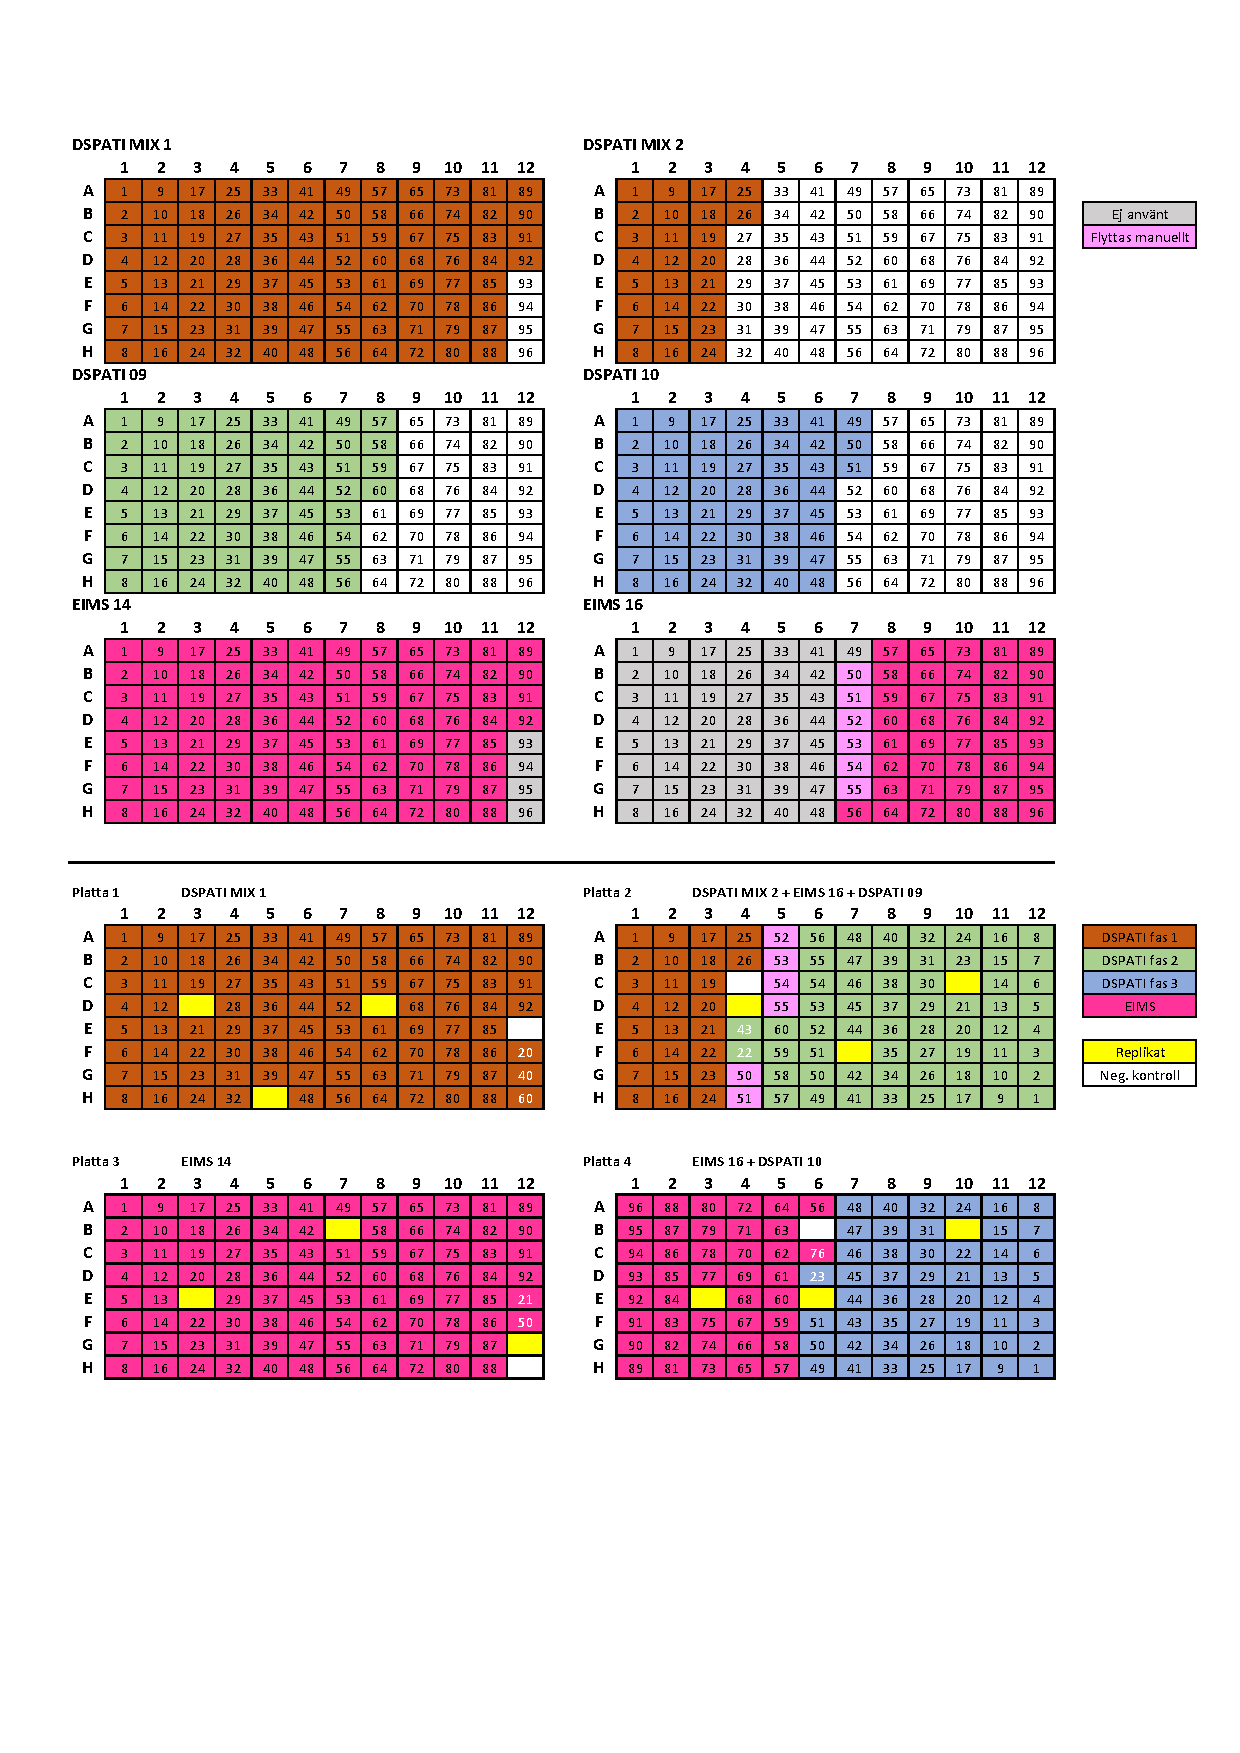
\includegraphics[clip, trim=0.5cm 5cm 0.5cm 2cm, width=\linewidth]{pages/AK prov layout.pdf}
\end{figure}

\newpage
\section{Extended group comparison results}\label{full_group_res}
\subsection{p-values and contingency values}
The following table shows all antigen called as significant for the comparison detailed in section \ref{method_group_comp}. Column p is the p-value obtained from Fisher's Exact Test when comparing the current phase of Covid patients to the EIMS controls, where green indicates a value below 0.0025 and yellow indicates a value below 0.05. The column n/N n/N denotes the number or reactive samples (n) and non-reactive samples (N) among the Covid patients and EIMS controls respectively. The columns kw1 and kw2 represent flagging of immunological function and extracellular localization, respectively, based on the Gene Ontology keywords detailed in appendix \ref{kw}.

The entries are divided in three groups which are explained in section \ref{method_group_comp} and explored in section \ref{res_group_comp}.

\begin{figure}[H]
	\centering
	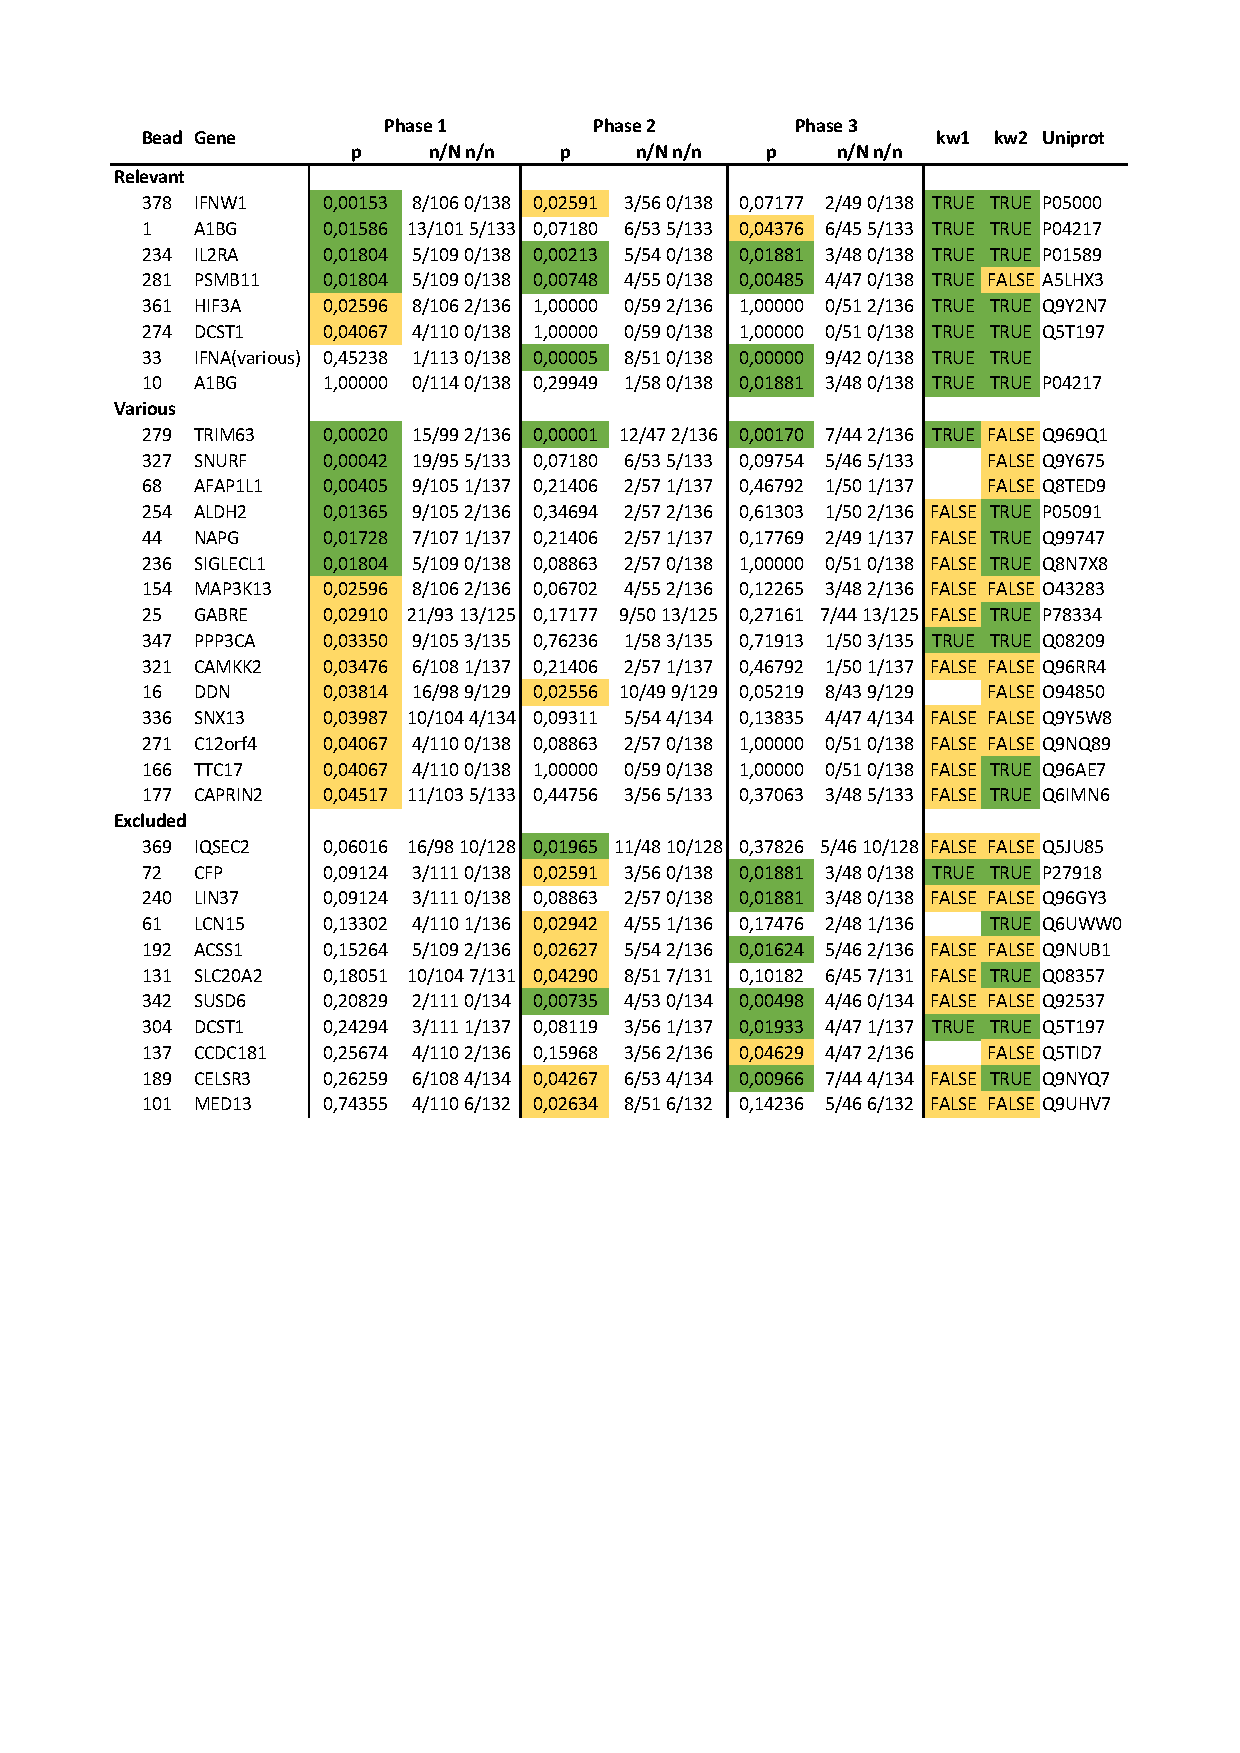
\includegraphics[clip, trim=1.8cm 10.5cm 1.8cm 2cm, width=\linewidth]{pages/sba_sig.pdf}
\end{figure}

\subsection{Additional plots}\label{gucci_various}
The same plots as in figure \ref{gucci_relevant} but for the various antigens.

\newpage
\begin{figure}[H]
	\centering
	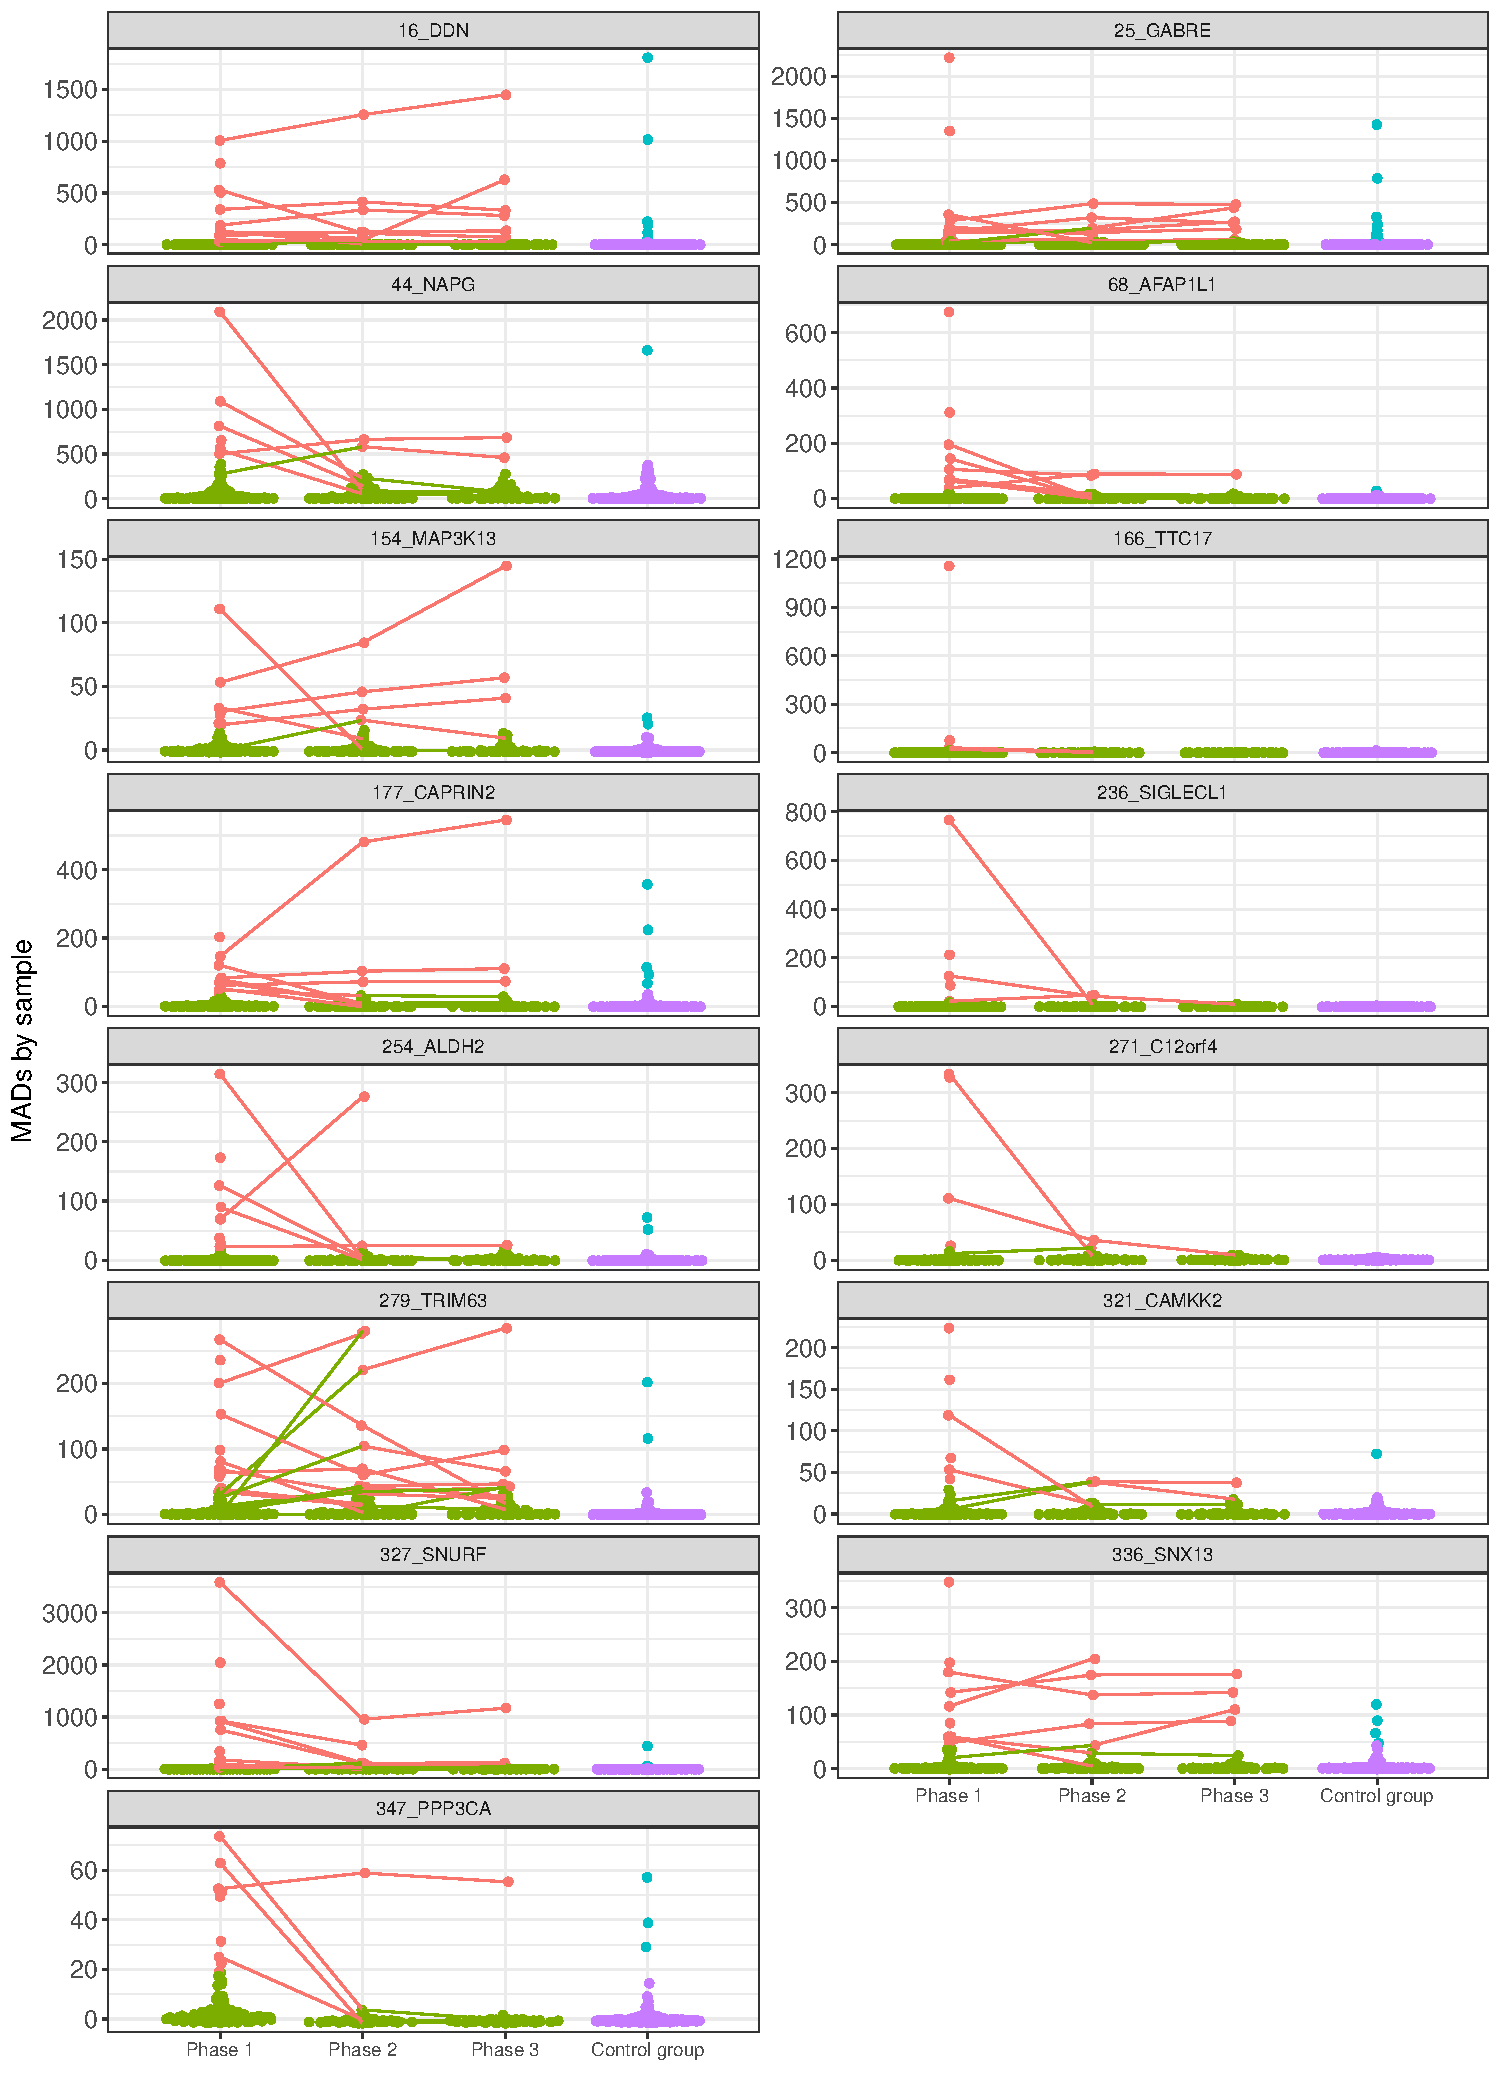
\includegraphics[width=0.95\linewidth]{figures/gucci_various+undoc.pdf}
\end{figure}

\newpage
\section{Planar microarray results}\label{42k_results}
The following are the significant results of the planar microarray analysis, containing 352 observations with a reactivity above 4 SDs.

The columns indicate the following:
\begin{enumerate}
    \item HPRR: The identifier of the PrEST as a bioinformatical construct.
    \item db: The percentage of the previous in-house runs in which the spot is deemed reactive.
    \item SDs: The normalized signal, as described in equation \ref{sds}.
    \item MFI: The pixel median fluorescence intensity of the spot foreground.
    \item p\_rank: Descending rank of the SDs of the current pool.
    \item Pool: Current pool.
    \item set: States which of the two glasses making up the microarray the observation occurred on.
    \item kw1: Gene ontology biological process was flagged as containing keywords in \ref{kw}.
    \item kw2: Gene ontology cellular compartment was flagged as containing keywords in \ref{kw}.
    \item Gene: HGNC gene identifier.
    \item Uniprot: Uniprot identifier
\end{enumerate}

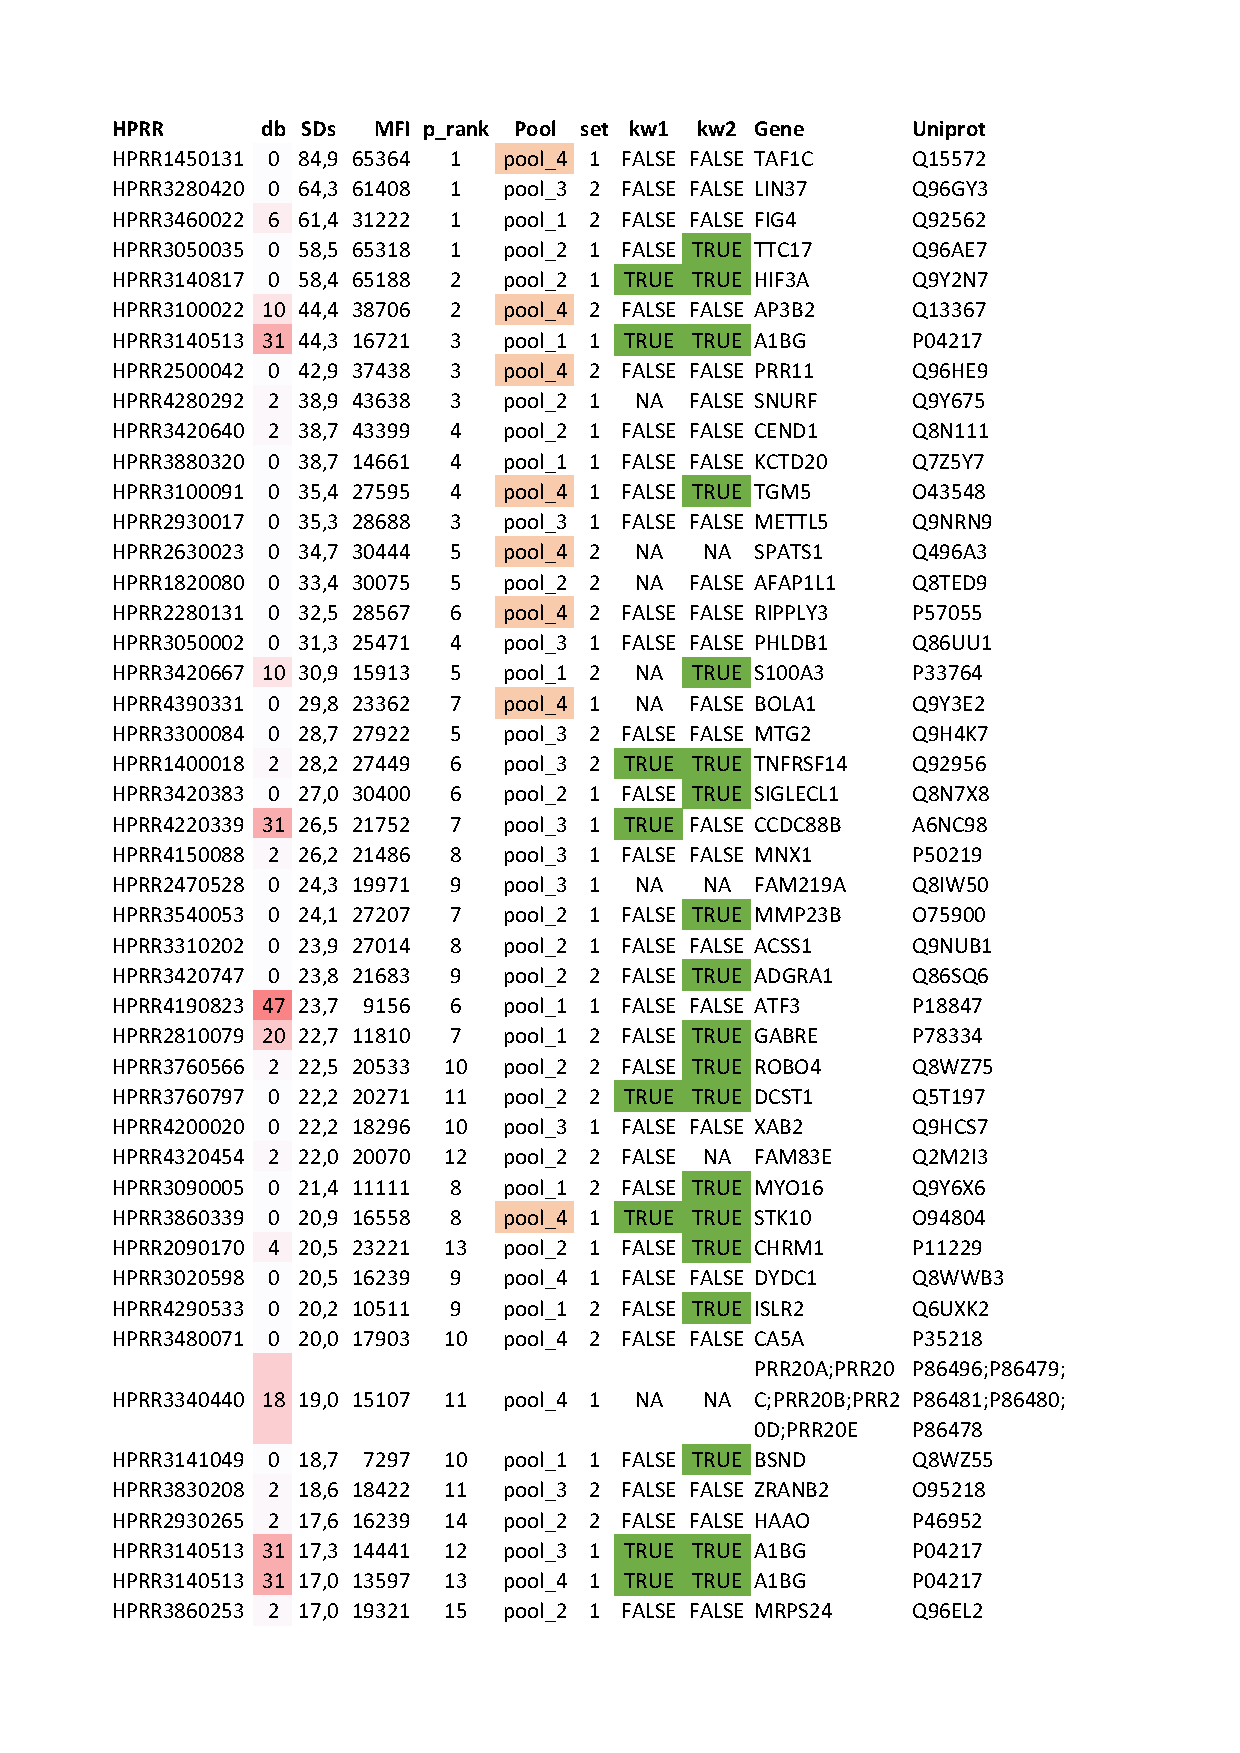
\includepdf[pages={1-8}, pagecommand={}, offset=1cm 1cm]{pages/42k_results.pdf}

\section{Suspension bead array}\label{sba_full}
\begin{figure}[H]
	\centering
	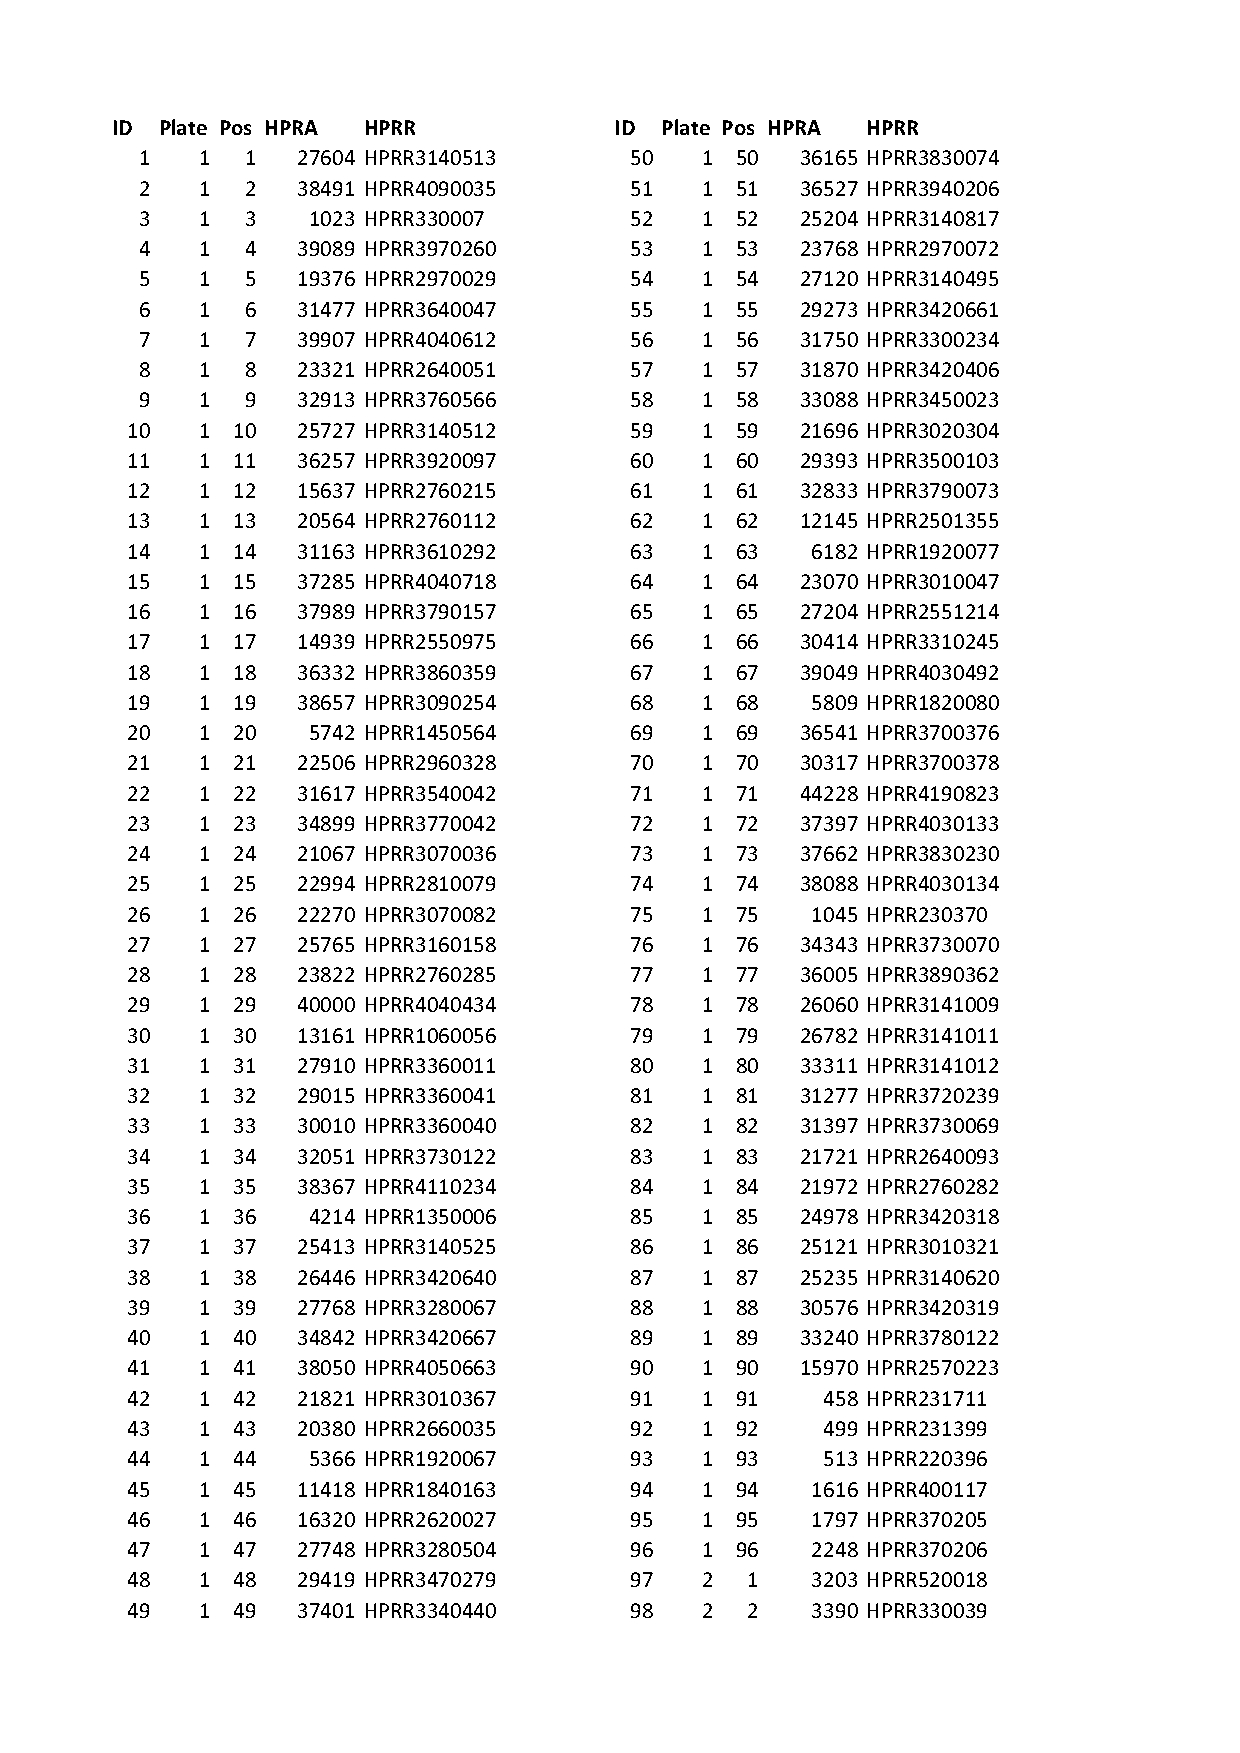
\includegraphics[clip, trim=1.8cm 2.3cm 1.8cm 2cm, width=0.92\linewidth]{pages/AK_SBA.pdf}
\end{figure}
\includepdf[pages={2-4}, pagecommand={}, offset=0cm 0cm, width=1.1\linewidth]{pages/AK_SBA.pdf}

\section{Code}
\subsection{Planar microarray data analysis}\label{code_42k}
\inputminted[linenos=true, frame=topline, label=42k\_analysis.R]{r}{code/42k_analysis.R}
\inputminted[linenos=true, frame=topline, label=42k\_plot.R]{r}{code/42k_plot.R}

\subsection{Compiling antigen panel information for localization}\label{panel_localize}
\inputminted[linenos=true, frame=topline, label=panel\_position\_input.R]{r}{code/panel_position_input.R}
\inputminted[linenos=true, frame=topline, label=panel\_sort\_output.R]{r}{code/panel_sort_output.R}

\subsection{Pre-run assay tests data analysis}\label{code_tests}
\inputminted[linenos=true, frame=topline, label=test\_analysis.R]{r}{code/test_analysis.R}

\subsection{Finding appropriate control plates}\label{code_control_wrangle}
\inputminted[linenos=true, frame=topline, label=MSC\_6\_wrangle.R]{r}{code/MSC_6_wrangle.R}

\subsection{SBA data analysis}\label{code_sba}
\inputminted[linenos=true, frame=topline, label=sba\_analysis.R]{r}{code/sba_analysis.R}
\inputminted[linenos=true, frame=topline, label=sba\_plot\_old.R]{r}{code/sba_plot_old.R}
\inputminted[linenos=true, frame=topline, label=sba\_plot\_results.R]{r}{code/sba_plot_results.R}

%\newpage
%\thispagestyle{empty}
%\mbox{}

\includepdf[pages={2}]{pages/cover.pdf}
\end{document}
